% REMEMBER: You must not plagiarise anything in your report. Be extremely careful.

\documentclass{l4proj}


%
% put any additional packages here
%
\usepackage{bm}
\usepackage{booktabs}
\usepackage{graphicx}
\usepackage[export]{adjustbox}

\begin{document}

%==============================================================================
%% METADATA
\title{Deep neural networks for classification of multispectral images}
\author{Niklas Lindorfer}
\date{September 26, 2019}

\maketitle

%==============================================================================
%% ABSTRACT
\begin{abstract}
    Every abstract follows a similar pattern. Motivate; set aims; describe work; explain results.
    \vskip 0.5em
    ``XYZ is bad. This project investigated ABC to determine if it was better. 
    ABC used XXX and YYY to implement ZZZ. This is particularly interesting as XXX and YYY have
    never been used together. It was found that  
    ABC was 20\% better than XYZ, though it caused rabies in half of subjects.''
\end{abstract}

%==============================================================================

% EDUCATION REUSE CONSENT FORM
% If you consent to your project being shown to future students for educational purposes
% then insert your name and the date below to  sign the education use form that appears in the front of the document. 
% You must explicitly give consent if you wish to do so.
% If you sign, your project may be included in the Hall of Fame if it scores particularly highly.
%
% Please note that you are under no obligation to sign 
% this declaration, but doing so would help future students.
%
\def\consentname {Niklas Lindorfer} % your full name
\def\consentdate {26 September 2019} % the date you agree
%
\educationalconsent


%==============================================================================
\tableofcontents

%==============================================================================
%% Notes on formatting
%==============================================================================
% The first page, abstract and table of contents are numbered using Roman numerals and are not
% included in the page count. 
%
% From now on pages are numbered
% using Arabic numerals. Therefore, immediately after the first call to \chapter we need the call
% \pagenumbering{arabic} and this should be called once only in the document. 
%
% The first Chapter should then be on page 1. You are allowed 40 pages for a 40 credit project and 20 pages for a 
% 20 credit report. This includes everything numbered in Arabic numerals (excluding front matter) up
% to but excluding the appendices and bibliography.
%
% You must not alter text size (it is currently 10pt) or alter margins or spacing.
%
%
%==================================================================================================================================
%
% IMPORTANT
% The chapter headings here are **suggestions**. You don't have to follow this model if
% it doesn't fit your project. Every project should have an introduction and conclusion,
% however. 
%
%==================================================================================================================================
\chapter{Introduction}

% reset page numbering. Don't remove this!
\pagenumbering{arabic} 


Why should the reader care about what are you doing and what are you actually doing?



%==================================================================================================================================
\chapter{Background}
What did other people do, and how is it relevant to what you want to do?

\section{Imaging}

\subsection{Electromagnetic radiation}

Visible light and infrared are forms of electromagnetic radiation. Visible light (VIS) has wavelengths roughly between $400$ and $700 nm$. The hue of visible light is determined by its wavelength. Colours as perceived by human vision are the result of a spectral distribution of wavelengths of the light than enters the eye. 

Infrared light (IR), with wavelengths between $700 nm$ and $1 mm$, is generally invisible to humans. It is commonly subdivided into near infrared (NIR), short-wavelength infrared (SWIR), medium-wavelength infrared (MWIR), long-wavelength infrared (LWIR), and far infrared (FIR) \citep[p. 28]{byrnes_unexploded_2008}, as can be seen in Figure \ref{fig:em_spectrum}.

\begin{figure}[ht]
  \centering
  \begin{subfigure}[h!]{0.9\textwidth}
    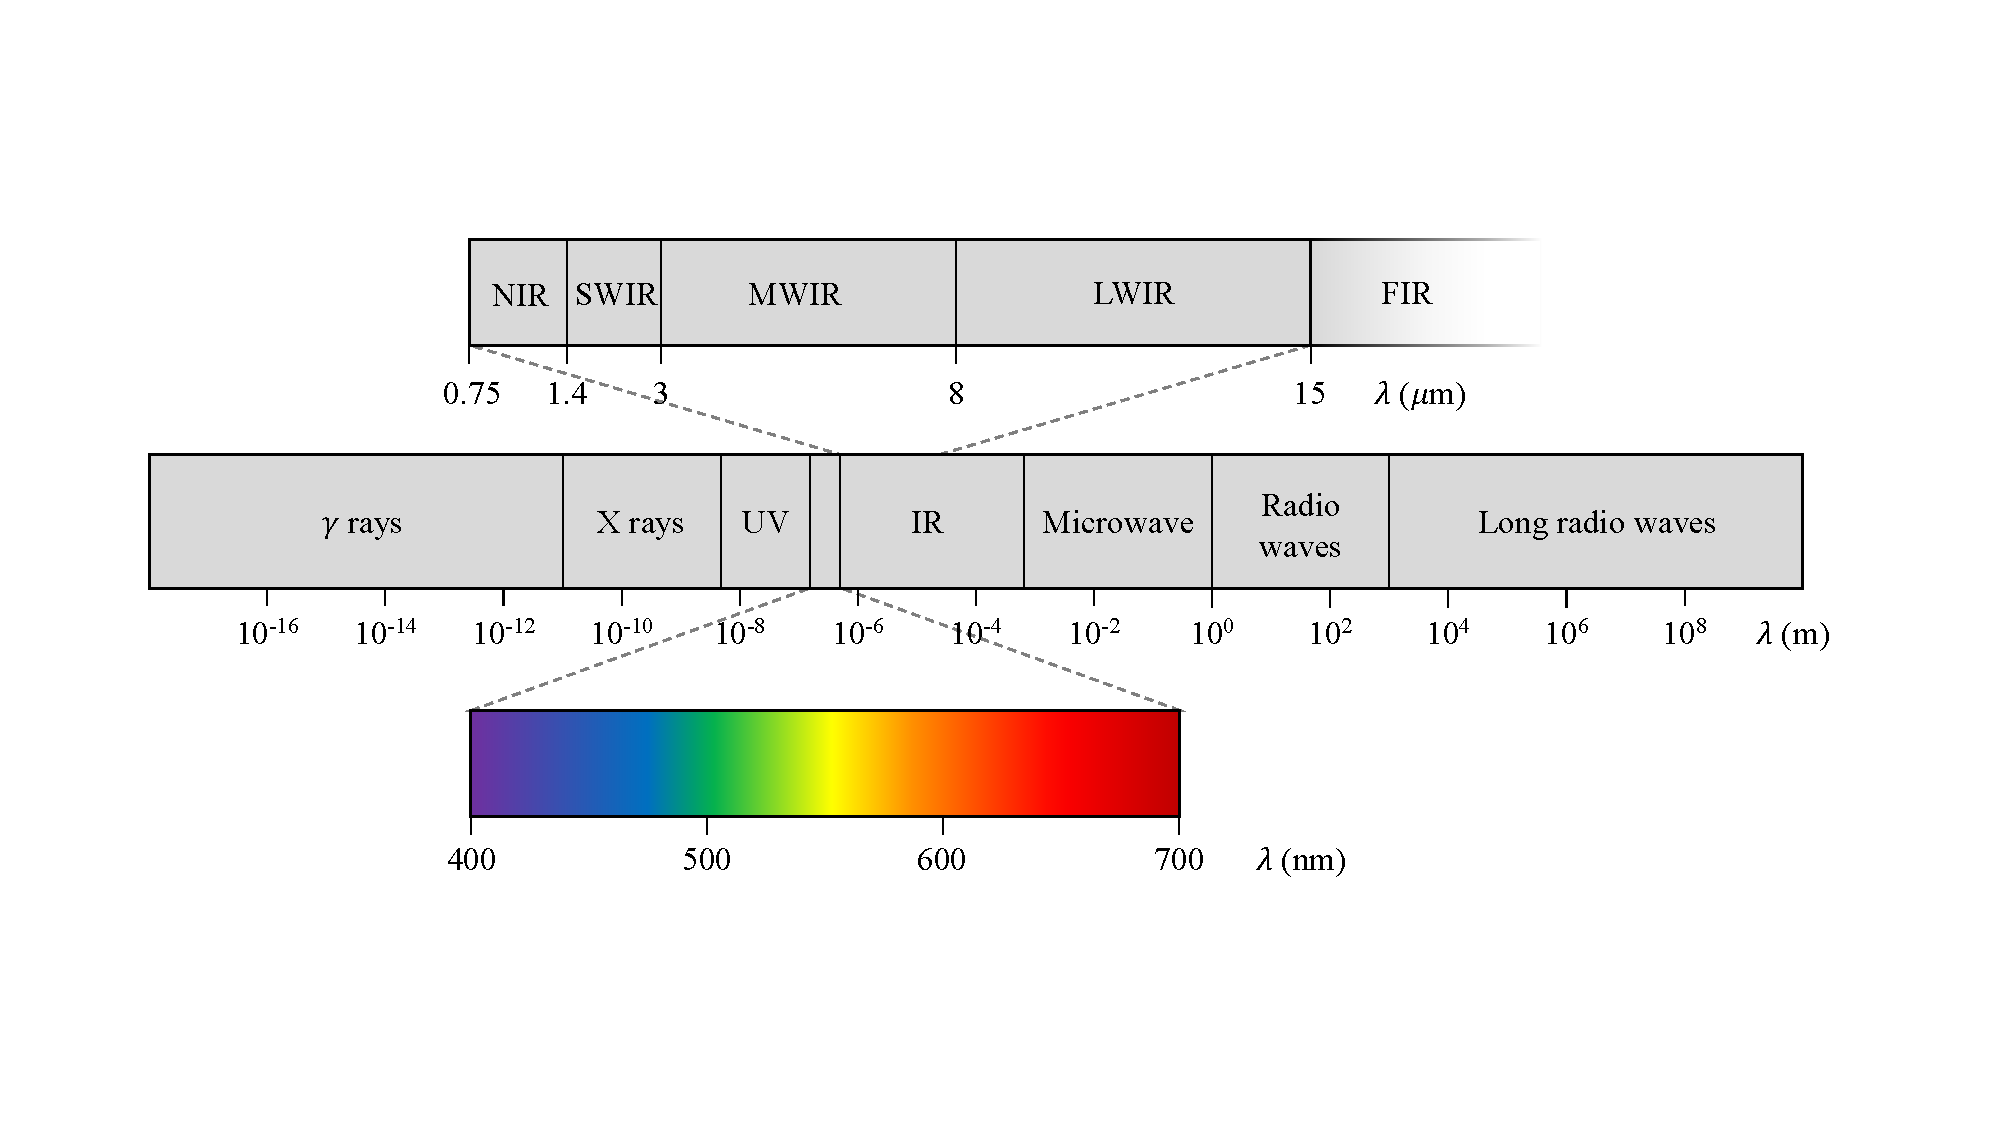
\includegraphics[width=\textwidth, trim={1.5cm 4cm 2cm 4cm}, clip=true]{images/EM_spectrum.pdf}
  \end{subfigure}
  \caption{The electromagnetic spectrum with detailled view of visible light and infrared. IR subdivisions modelled after \citet[p. 28]{byrnes_unexploded_2008}.}
  \label{fig:em_spectrum}
\end{figure}

\subsection{Thermal infrared radiation}

Black-body radiation is defined as thermal electromagnetic radiation emitted by an idealized opaque, non-reflective body \citep{young_sears_2012}. It has a continuous frequency spectrum that is dependent on the temperature of the body \citep{kogure_thermodynamic_2007}. The spectrum has a characteristic peak, which is antiproportional to the temperature $T [K]$ according to Wien's displacement law:

\begin{equation}
  \lambda_{peak} = \frac{2.898 \times 10^{-3}}{T} [m],
\end{equation}

Bodies at a room temperature of $300 K$ emit electromagnetic radiation with a peak at $9.7 \mu m$ \citep{jarc_graz_2007}, falling into the LWIR range. To account for different non-ideal surfaces, the material-specific emissivity constant $\epsilon \in [0..1]$ is introduced to describe the share of radiation that is emitted by a body compared to an ideal black body. The total energy radiated by a body per unit surface and time is expressed by the Stefan-Boltzmann law:

\begin{equation}
  W = \epsilon \sigma T^4,
\end{equation}

where $\sigma$ is a proportionality constant. Thus, if the emissivity of the body is known, this law can be applied to determine its temperature. This is the theoretical foundation for thermal imaging. In practice, the material and corresponding emissivity are often undetermined. Therefore, the received infrared radiation contains an unknown share of reflected radiation, adding noise to the measurement. This can be somewhat mitigated by estimating the value of $\epsilon$.

\subsection{Spectral imaging}

Spectral images combine spatial and spectral information in a 3-D data structure where the dimensions correspond to height, width and waveband. 
A distinction is made between hyperspectral and multispectral imaging techniques. 

If an image is acquired at many (tens or hundreds) regularly sampled wavebands, one speaks of a hyperspectral image, sometimes referred to as a hypercube. Hyperspectral images have many powerful applications, including agriculture and food quality \citep{dale_hyperspectral_2013} and medical applications \citep{lu_medical_2014}. However, capturing hyperspectral images requires advanced sensing equipment. Furthermore, hypercubes are difficult to process due to the high amount of information and therefore often require the application of computationally expensive preprocessing techniques, such as dimensionality-reduction \citep{qin_hyperspectral_2013}.

Multispectral images comprise of a few discrete wavebands. As opposed to hyperspectral images, it is usually not possible to extract a full continuous spectrum of an individual pixel from multispectral images \citep{abdul_multi-disnet_2019}.


%----------------------------------------------------------------------------------------------------------------------------------

\section{Machine learning}

\subsection{Supervised and unsupervised algorithms}

Machine learning techniques can be categorised into supervised, semi-supervised, unsupervised, and reinforcement learning \citep{burkov_hundred-page_2019}.

In supervised learning, a dataset consisting of a list of labelled features $\{(\vec{x}_i, y_i)\}^N_{i=1}$ is provided. $\vec{x_i}$ is called a feature vector. The supervised learning algorithm then attempts to fit a model $f$ on the dataset such that $\forall{\vec{x_i}}. (f(\vec{x_i}) = y_i)$. The model can then be used to predict the unknown label of a test data point. In practice, a perfect fit is not possible due to noise in the dataset. Therefore, supervised algorithms are evaluated according to a loss function measuring the difference between $f(\vec{x_i})$ and $y_i$. When fitting the model, the algorithm attempts to minimise the loss over the training data. Common choices for loss functions are mean squared error (MSE) for regression and categorical cross-entropy for classification problems.

Unsupervised learning involves a dataset of unlabeled data $\{\vec{x}_i\}^N_{i=1}$. An unsupervised learning algorithm attempts to transform each feature vector $\vec{x}_i$ into another vector to solve a practical problem, such as dimensionality reduction or outlier detection \citep{burkov_hundred-page_2019}. 
This project focuses on supervised learning.

\subsection{Regression and classification}

In supervised learning, one speaks of classification or regression, depending on whether the data labels $y_i$ are discrete classes or continous, real values.

\subsection{Deep learning}






%==================================================================================================================================

\chapter{Analysis/Requirements}
What is the problem that you want to solve, and how did you arrive at it?

\section{Data generation}

Collecting a multispectral dataset is significantly more challenging than a dataset consisting solely of visible-light images. The majority of image classification tasks use traditional imaging only (XXX citation needed). Consequently, the amount of research and resources available to use is much more limited.

\subsection{Transfer learning}

A large amount of existing datasets is available for traditional image classification tasks. The ImageNet dataset \citep{deng_imagenet_2009}, which is used as a benchmark for many image classification models, contains over a million images ready to be used. Many successful deep learning models, such as AlexNet \citep{krizhevsky_imagenet_2012} and ResNet \citep{he_deep_2016} have been applied to datasets such as ImageNet.

When creating a new image classifier, it is then possible to incorporate pretrained versions of these networks into a new classifier and perform transfer learning on a new dataset. This strategy makes it feasible to train complex models on smaller amounts of data than usual, as many meaningful weights have already been learned by the pretrained model (XXX citation needed).

For multispectral models, this approach becomes more difficult, as much fewer datasets are available to be used off-the-shelf. Datasets for visible light and thermal data, such as the KAIST Pedestrian Detection Benchmark \citep{hwang_multispectral_2015} are available. However, They usually lack the variety and size of traditional computer vision datasets and are therefore less suitable for general tasks.

Pre-training a multispectral classifier on an VIS-only dataset is not directly possible due to the incompatible input tensor shapes ($h \times w \times 3$ compared to $h \times w \times 4$) and the resulting difference in trainable weights.

However, there are strategies to mitigate this issue. It is possible to divide the model into 2 separate branches of layers that process the VIS and LWIR images individually, and perform late feature fusion by concatenating the respective feature maps and adding at least one fully connected layer after the concatenation. This approach would make it possible to load pretrained weights into the VIS-branch of the model without affecting the LWIR branch. During training, the LWIR-branch of the model would get trained from scratch, whereas transfer learning is simultaneously performed on the VIS-branch.

Another possible approach to enable the usage of existing off-the-shelf datasets is to perform generative image augmentation. In Section \ref{autoencoder_implementation} we explore the application of a primitive generative model for predicting the corresponding LWIR image of a known type of object from a given RGB image. Given sufficient quality of predicted images, it would then be possible to turn RGB-only images into multispectral training data.


\subsection{Sensory equipment}

Even though thermal cameras have become significantly more affordable in recent years, their resolution remains much lower than that of conventional visible-light cameras. The FLIR One Pro, which was used for this project, is composed of two sensors:

\begin{itemize}
  \item A conventional camera for visible-light images with a resolution of $1440 \times 1080$ px.
  \item A thermal sensor with a resolution of $160 \times 120$ px and a spectral range of $8 - 14 \mu m$.
\end{itemize}

The sensor is therefore able to perceive and record electromagnetic waves in the visible-light (VIS) and long wave infrared (LWIR) bands. Due to technical limitations, several challenges had to be overcome when working with data collected by the sensor.

Firstly, the two cameras are not spatially aligned. Furthermore, the "zoom level" or focal length of the sensors does not appear to match. A misalignment of the channels is likely to have an impact on the performance of a convolutional network (XXX citation needed). Therefore, the issue of image registration of the two camera outputs arises. The strategy we introduced to perform robust registration is outlined in Section \ref{image_registration}.

Secondly, the vastly different resolutions of the sensors could cause problems, as convolutional filters might struggle detecting edges and other features (XXX).

%----------------------------------------------------------------------------------------------------------------------------------

\section{Mobile application}

This project aims to deploy the final deep learning model to a mobile edge device. This introduces many challenges related to mobile computing. Contrary to most computers, computational power on mobile devices is highly limited. Furthermore, to provide robust and reliable real-time classification, low latency between image capture and classification will be necessary. Two major strategies can be used to apply image classification on a mobile device:

\begin{enumerate}
  \item Deploy the model to a web service, upload captured frames from edge device, and retrieve the prediction.
  \item Deploy the model to the edge device and perform all computations "offline".
\end{enumerate}

To minimise latency, the second approach was selected. It will therefore be possible to use the application even in situations with poor connectivity. However, the necessity to perform all computational tasks on the edge-device imposes many problems. The Tensorflow SDK for Java is very limited compared to the Python API. Furthermore, various image pre-processing tasks have to be performed without the standard Python data science stack that was used for training and experimentation. Many image processing libraries do not support multispectral data, further complicating image processing.

The mobile application will furthermore provide the ability to capture datasets in a convenient way, without the need to seperately extract raw RGB and LWIR images after capture.


%==================================================================================================================================
\chapter{Design}
How is this problem to be approached, without reference to specific implementation details? 


\section{Dataset}

\subsection{Classes and samples}
\label{classes_samples}

Initially, a dataset consisting of 13 classes and 1042 samples was captured using the camera functionality of the mobile application. The app captures images in quick temporal succession, effectively like a video. Thus, many images are relatively similiar, as they were captured within only a few milliseconds difference. To distinguish between different "bursts" of images, images were grouped into distinct subsets, each subset representing a batch of similar images.

Due to the difficulty of obtaining well-framed and unobstructed images, the data contains some noise. Some images contain more than one animal. Furthermore, some animals were housed in closed-off shelters and were only visible behind a metal grid. Therefore, each subset was labeled as either \textit{single}, \textit{multi}, or \textit{obstructed}, to allow greater flexibility when selecting data for training and validation. Moreover, no distinction between genders was made. This primarily impacts the peacock class, as male and female peacocks have a very distinct appearance.

\begin{table}[ht]
  \centering
  \begin{tabular}{@{}llll@{}}
    \toprule
    \textbf{Class}  & \textbf{Dataset 1} & \textbf{Dataset 2} & \textbf{Dataset 3}  \\ \midrule
    Cat             & 205              & 0                    & 0                   \\ 
    Pig             & 30               & 0                    & 0                   \\
    Pony            & 112              & 127                  & 234                 \\
    Sheep           & 36               & 0                    & 0                   \\
    Alpaca          & 85               & 391                  & 115                 \\
    Ferret          & 33               & 0                    & 0                   \\
    Peacock         & 157              & 79                   & 0                   \\
    Hamburg chicken & 29               & 58                   & 49                  \\
    Silkie chicken  & 17               & 129                  & 83                  \\
    Muscovy duck    & 24               & 141                  & 105                 \\
    Chicken         & 138              & 151                  & 170                 \\
    Rabbit          & 32               & 16                   & 0                   \\
    Goose           & 144              & 0                    & 0                   \\ \bottomrule
  \end{tabular}
  \caption{Classes and sample size of raw animals datasets.}
  \label{table:raw_dataset}
\end{table}

Initially, the separation into training and validation data was performed using a stratified random split of all the data. As demonstrated in Section \ref{eval_train_val_split}, nearly perfect validation accuracy was achieved on this split. This most likely being a result of the aforementioned similarity of many images due to them being captured at similar times, we decided that a second, independent dataset was necessary to achieve representative evaluation results. The classes and samples of both datasets are shown in Table \ref{table:raw_dataset}.

Finally, the subsets from both datasets were rearranged into a training dataset and a testing dataset. An attempt was made to obtain a balanced mixture of \textit{single}, \textit{multi}, and \textit{obstructed} subsets in both datasets. Nonetheless, it can be assumed that achieving a perfect, representative split is difficult due to the noise in the dataset and the limited variety of contexts. The train-test-split is shown in Table \ref{table:train_test_dataset}.


\begin{table}[ht]
  \centering
  \begin{tabular}{@{}lll@{}}
    \toprule
    \textbf{Class}  & \textbf{Train } & \textbf{Test} \\ \midrule
    Cat             & 149             & 56 \\
    Pony            & 415             & 58 \\
    Alpaca          & 377             & 87 \\
    Peacock         & 157             & 79 \\
    Hamburg chicken & 77              & 59 \\
    Silkie chicken  & 191             & 38 \\
    Muscovy duck    & 206             & 64 \\
    Chicken         & 277             & 119 \\
    Goose           & 125             & 19 \\ \bottomrule
  \end{tabular}
  \caption{Classes and sample size train and test datasets.}
  \label{table:train_test_dataset}
\end{table}

The classes with low support (Pig, Sheep, Ferret, Rabbit) were dropped from the datasets, as it was deemed unlikely that a model would be able to accurately be fit on such small numbers of samples. A problem that remained is the class imbalance in both datasets. Alpacas are over-represented and Hamburg chicken are significantly under-represented.

\begin{figure}[ht]
  \centering
  \begin{subfigure}[h!]{0.18\textwidth}
    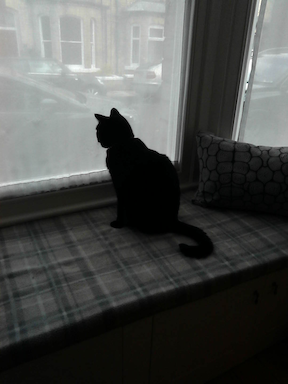
\includegraphics[width=\textwidth, trim={0cm 6cm 0cm 6cm}, clip]{images/dataset/cat/rgb.png}
    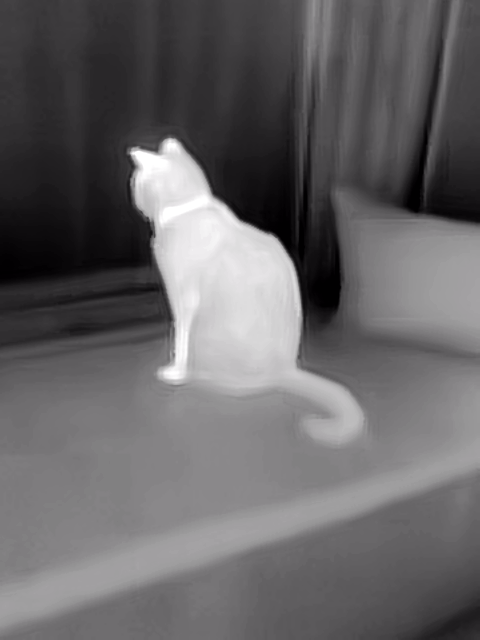
\includegraphics[width=\textwidth, trim={0cm 2.5cm 0cm 2.5cm}, clip]{images/dataset/cat/lwir.png}
    \caption{Cat}
  \end{subfigure}
  \begin{subfigure}[h!]{0.18\textwidth}
    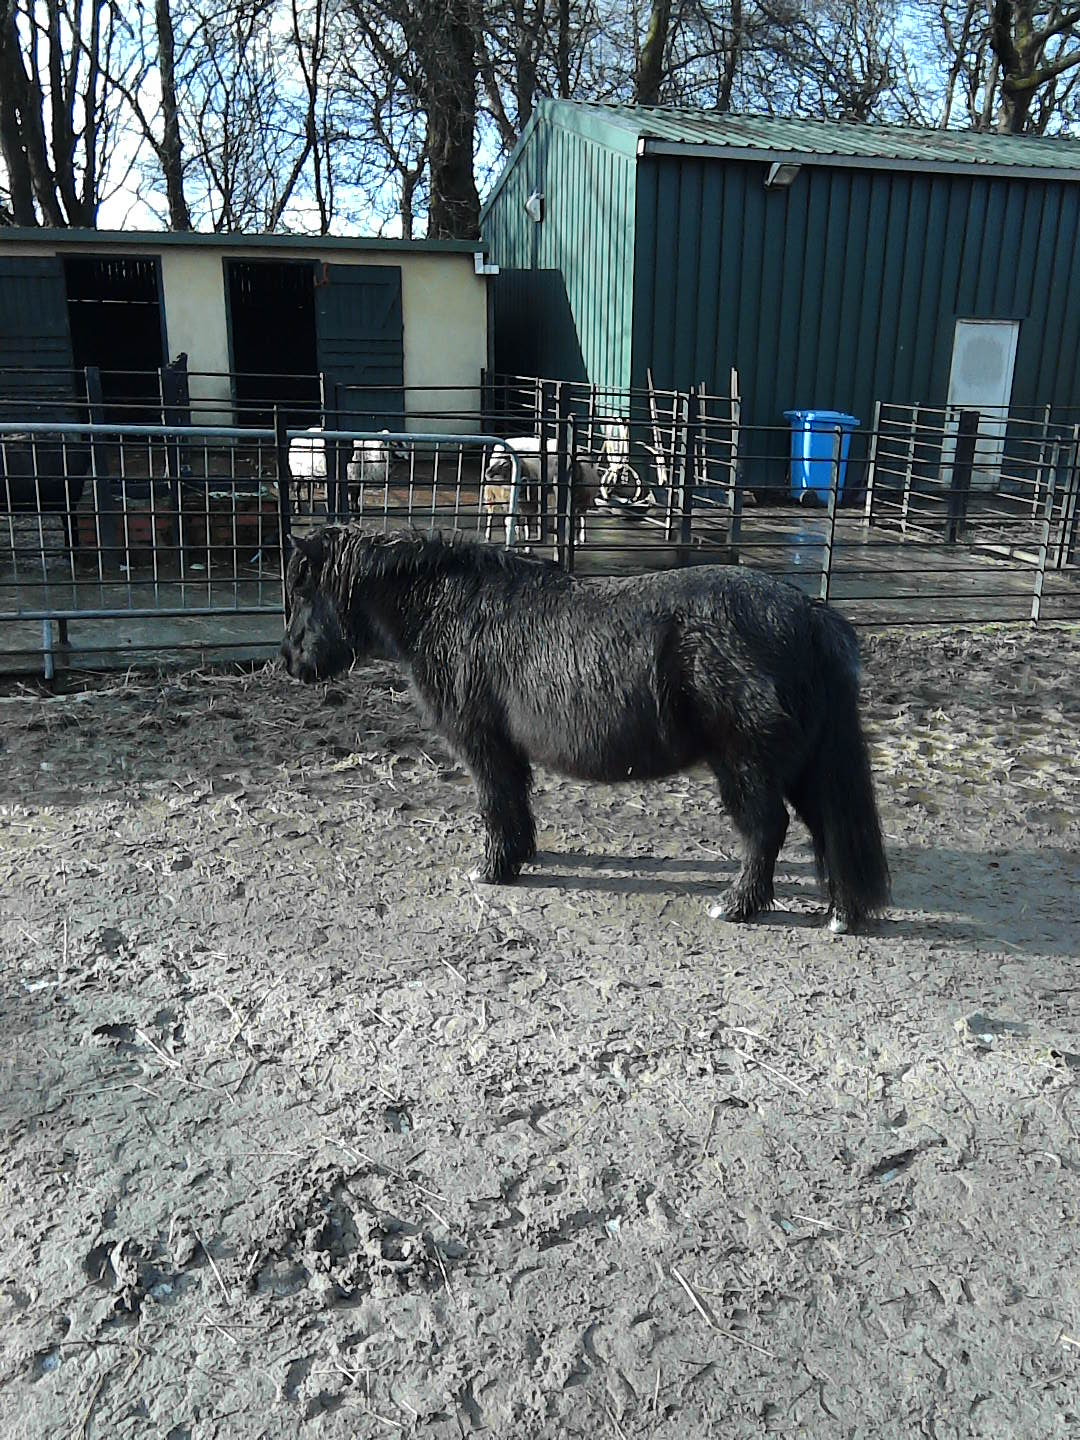
\includegraphics[width=\textwidth, trim={0cm 6cm 0cm 6cm}, clip]{images/dataset/pony/rgb.png}
    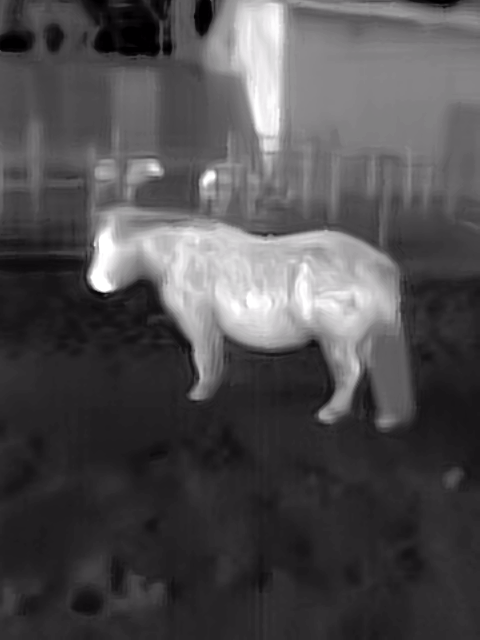
\includegraphics[width=\textwidth, trim={0cm 2.5cm 0cm 2.5cm}, clip]{images/dataset/pony/lwir.png}
    \caption{Pony}
  \end{subfigure}
  \begin{subfigure}[h!]{0.18\textwidth}
    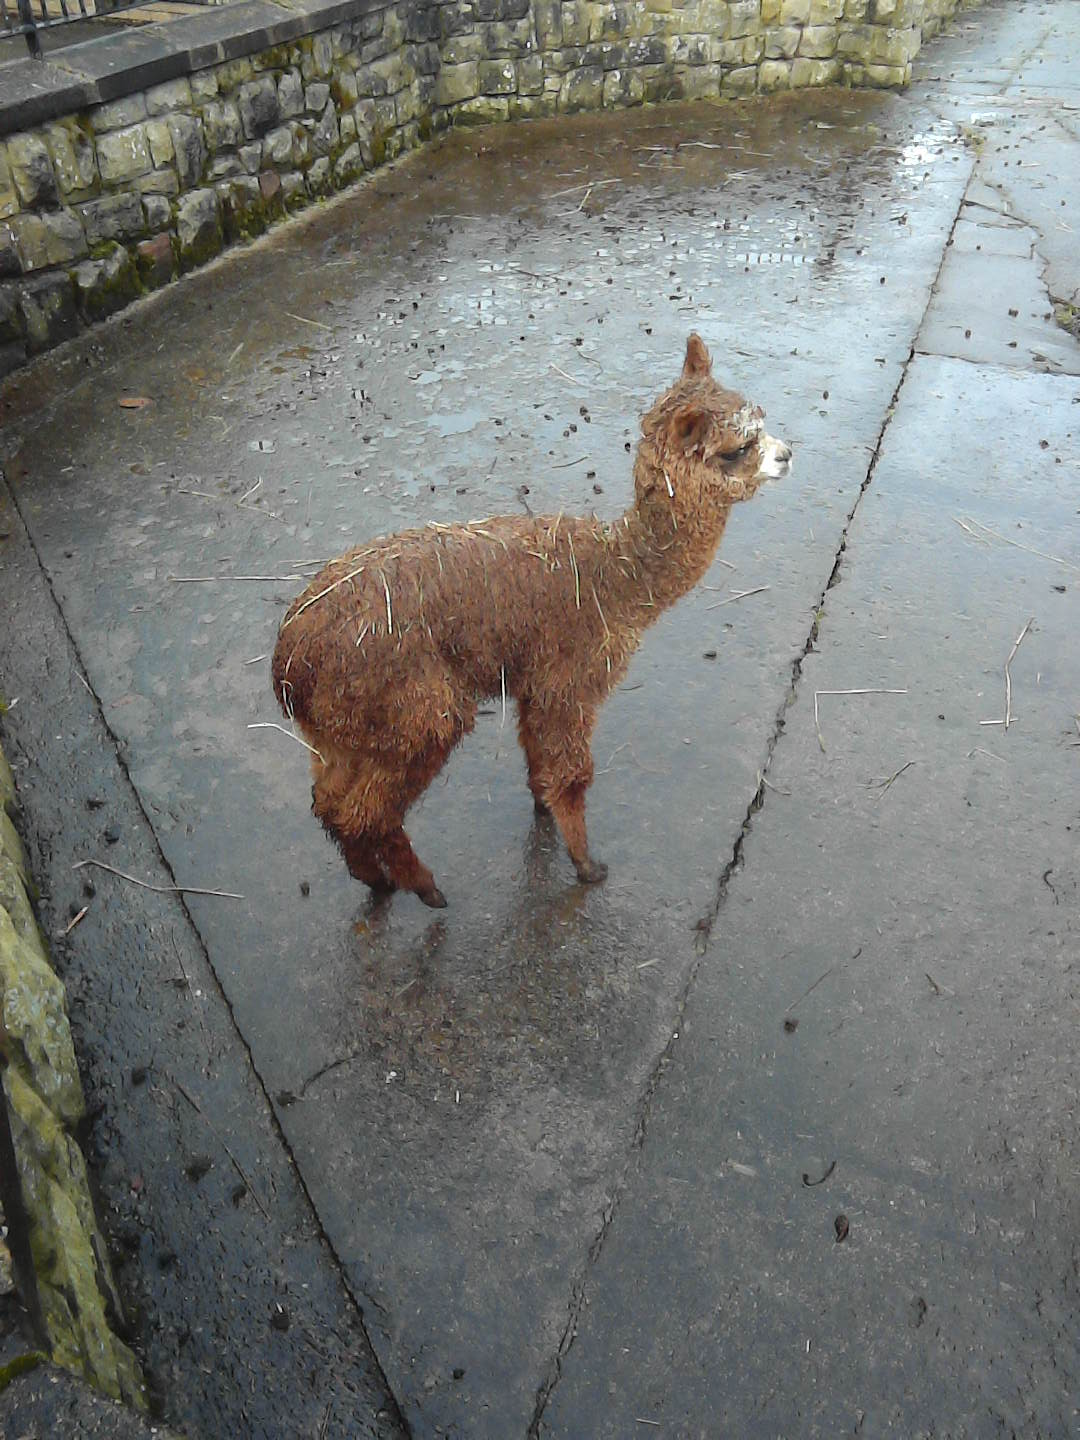
\includegraphics[width=\textwidth, trim={0cm 6cm 0cm 6cm}, clip]{images/dataset/alpaca/rgb.png}
    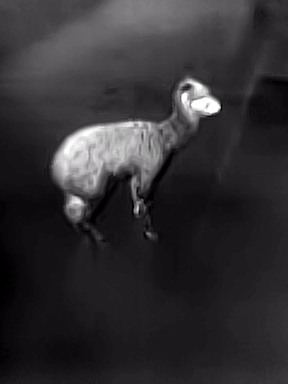
\includegraphics[width=\textwidth, trim={0cm 2.5cm 0cm 2.5cm}, clip]{images/dataset/alpaca/lwir.png}
    \caption{Alpaca}
  \end{subfigure}
  \begin{subfigure}[h!]{0.18\textwidth}
    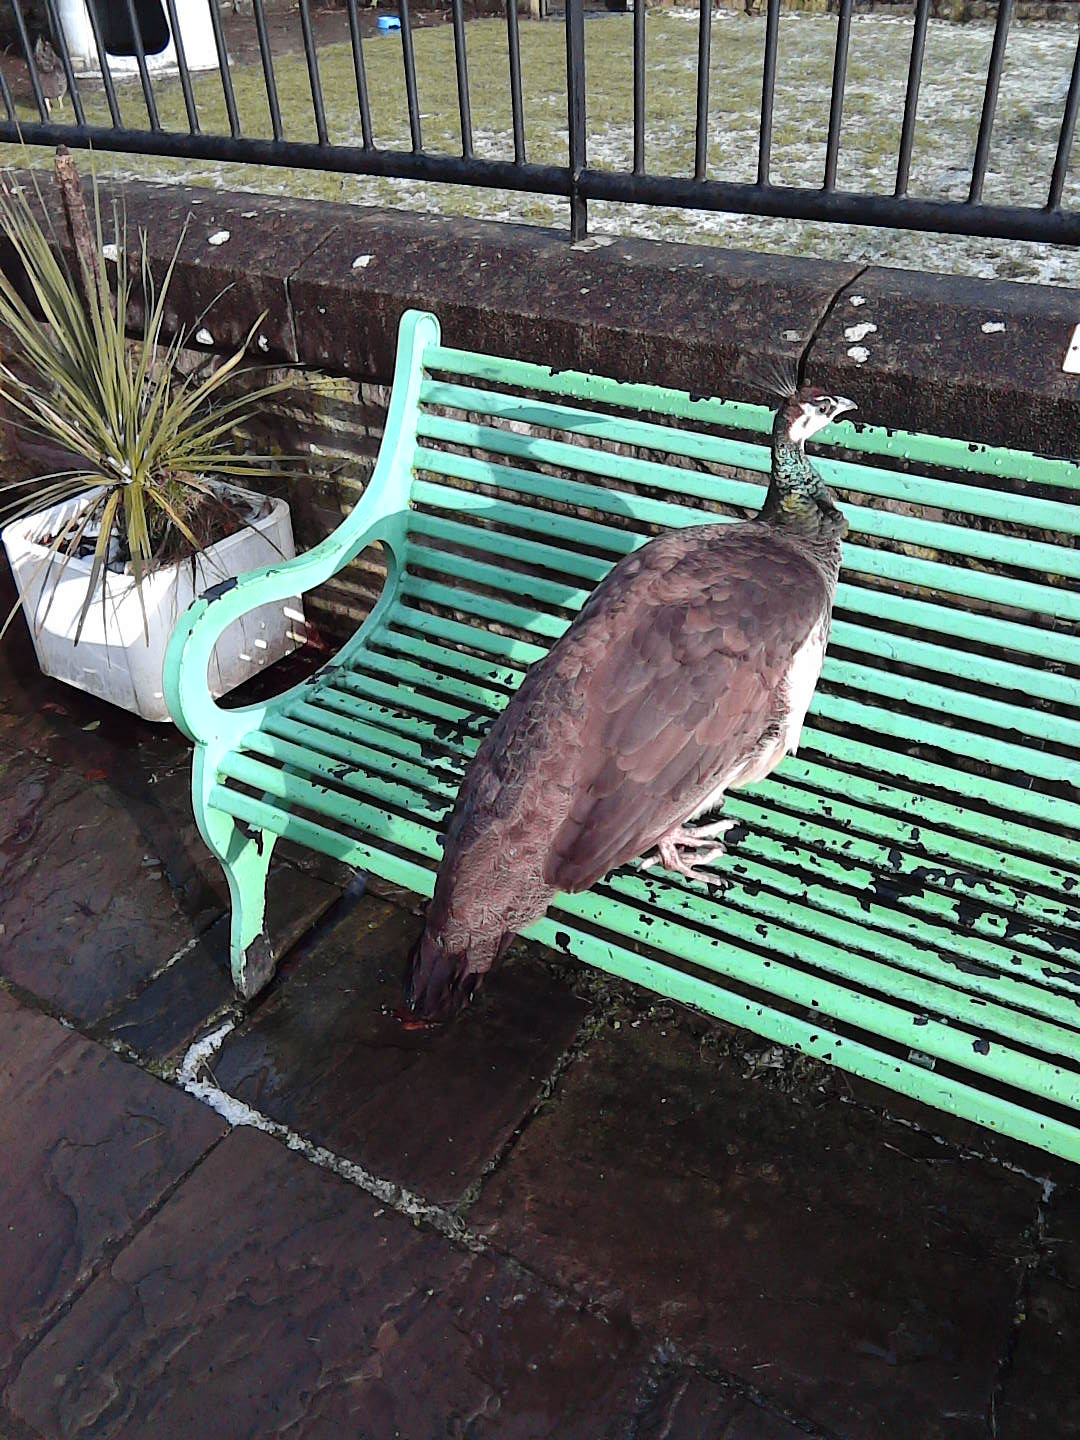
\includegraphics[width=\textwidth, trim={0cm 6cm 0cm 6cm}, clip]{images/dataset/peacock/rgb.png}
    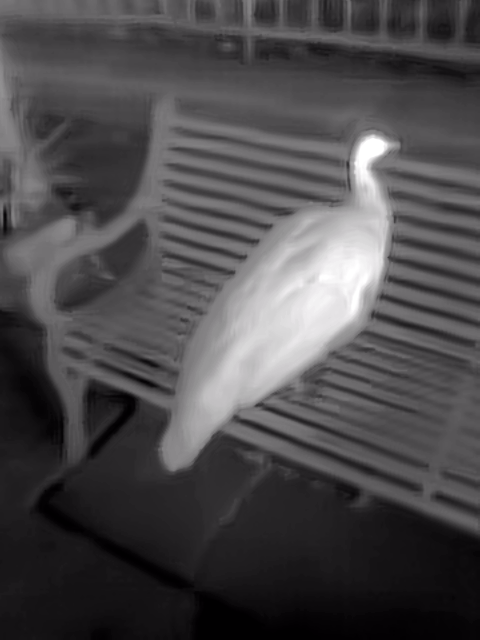
\includegraphics[width=\textwidth, trim={0cm 2.5cm 0cm 2.5cm}, clip]{images/dataset/peacock/lwir.png}
    \caption{Peacock}
  \end{subfigure}
  \begin{subfigure}[h!]{0.18\textwidth}
    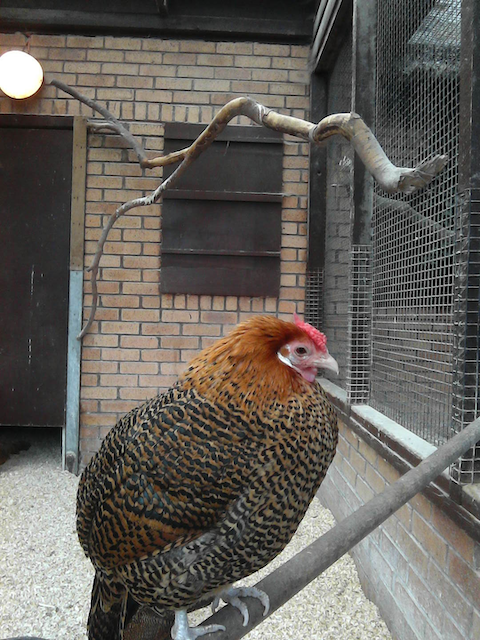
\includegraphics[width=\textwidth, trim={0cm 6cm 0cm 6cm}, clip]{images/dataset/pretty_chicken/rgb.png}
    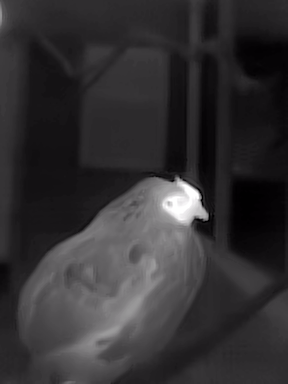
\includegraphics[width=\textwidth, trim={0cm 2.5cm 0cm 2.5cm}, clip]{images/dataset/pretty_chicken/lwir.png}
    \caption{Hamburg chicken}
  \end{subfigure}
  \begin{subfigure}[h!]{0.18\textwidth}
    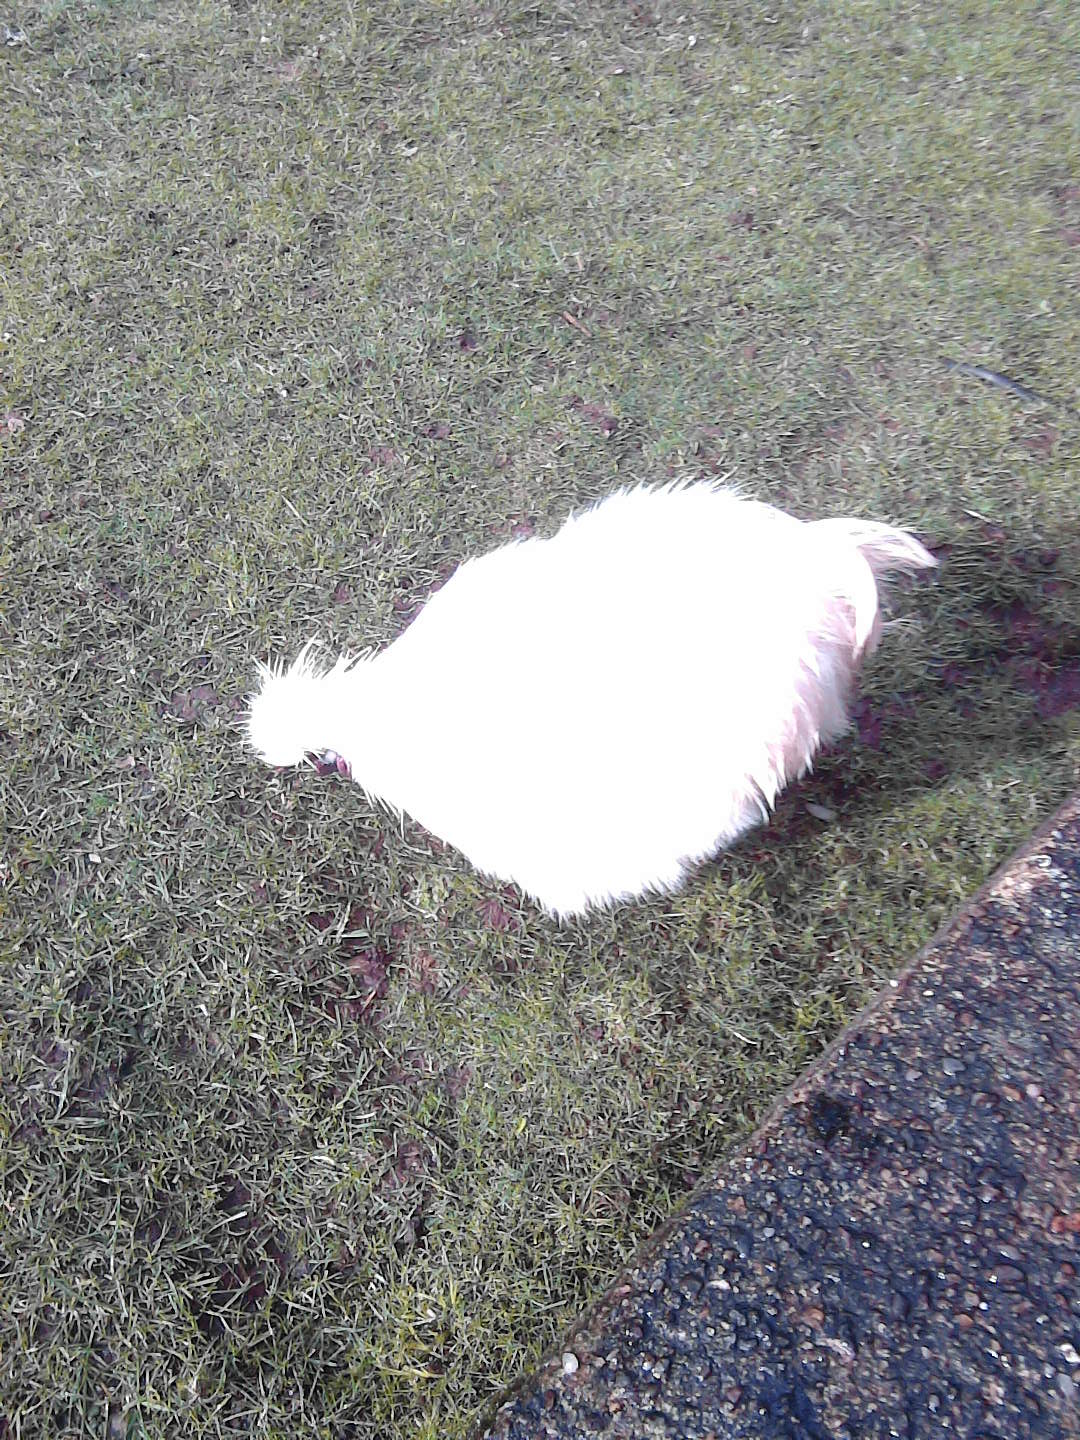
\includegraphics[width=\textwidth, trim={0cm 6cm 0cm 6cm}, clip]{images/dataset/evil_chicken/rgb.png}
    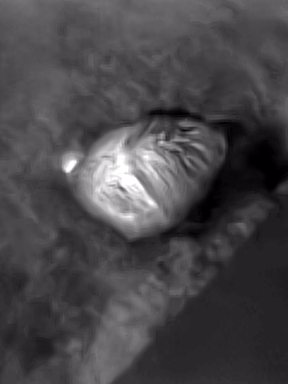
\includegraphics[width=\textwidth, trim={0cm 2.5cm 0cm 2.5cm}, clip]{images/dataset/evil_chicken/lwir.png}
    \caption{Evil chicken}
  \end{subfigure}
  \begin{subfigure}[h!]{0.18\textwidth}
    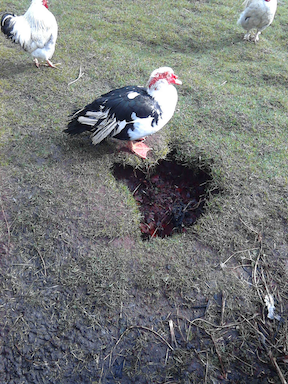
\includegraphics[width=\textwidth, trim={0cm 6cm 0cm 6cm}, clip]{images/dataset/ugly_duck/rgb.png}
    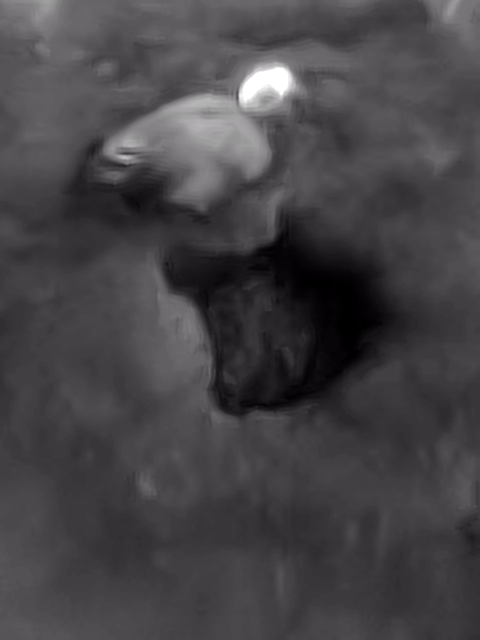
\includegraphics[width=\textwidth, trim={0cm 2.5cm 0cm 2.5cm}, clip]{images/dataset/ugly_duck/lwir.png}
    \caption{Ugly duck}
  \end{subfigure}
  \begin{subfigure}[h!]{0.18\textwidth}
    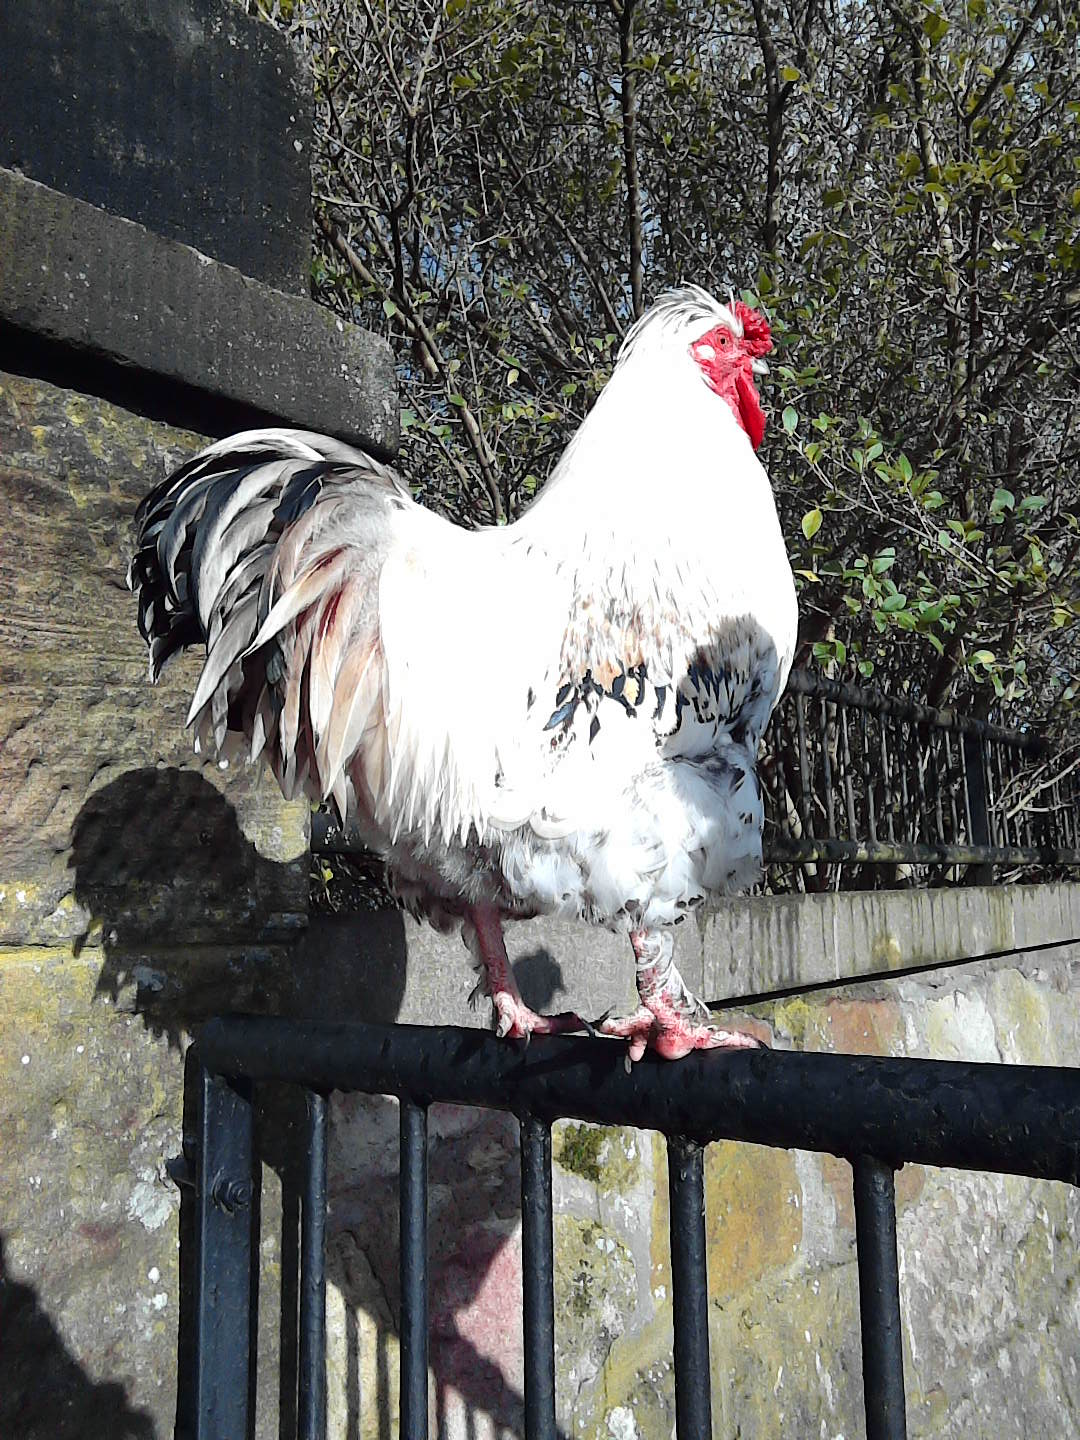
\includegraphics[width=\textwidth, trim={0cm 6cm 0cm 6cm}, clip]{images/dataset/chicken/rgb.png}
    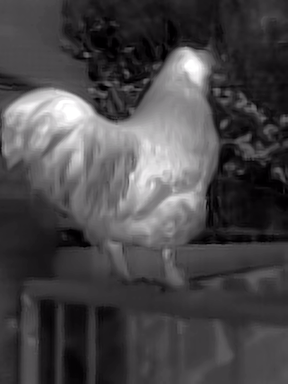
\includegraphics[width=\textwidth, trim={0cm 2.5cm 0cm 2.5cm}, clip]{images/dataset/chicken/lwir.png}
    \caption{Chicken}
  \end{subfigure}
  \begin{subfigure}[h!]{0.18\textwidth}
    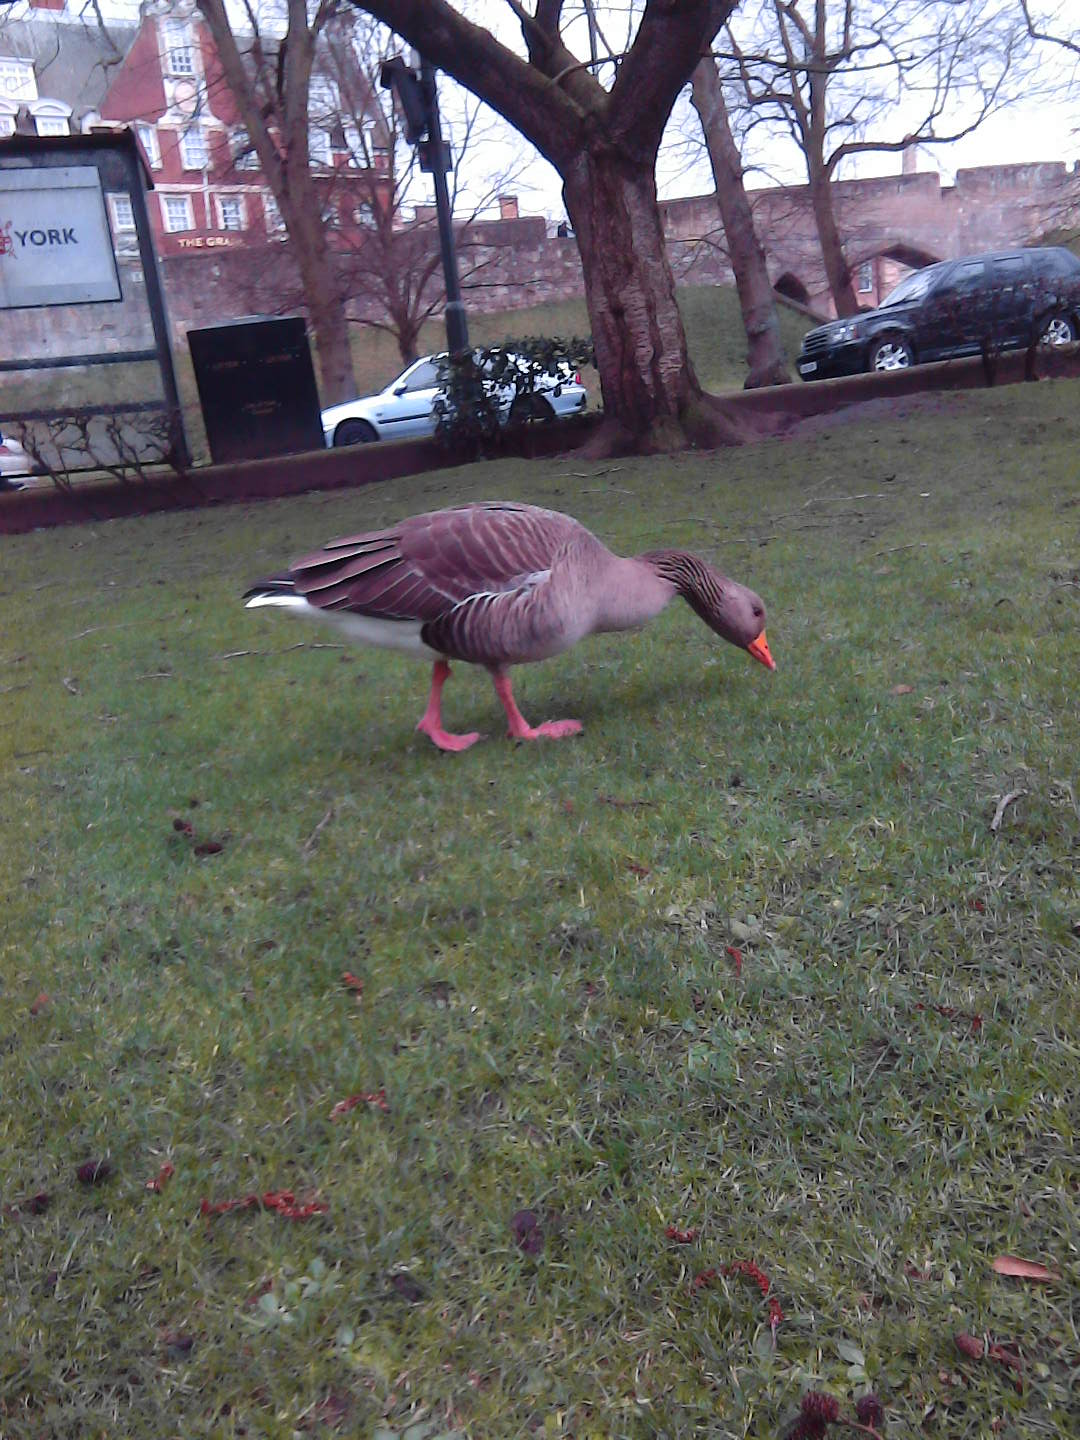
\includegraphics[width=\textwidth, trim={0cm 6cm 0cm 6cm}, clip]{images/dataset/goose/rgb.png}
    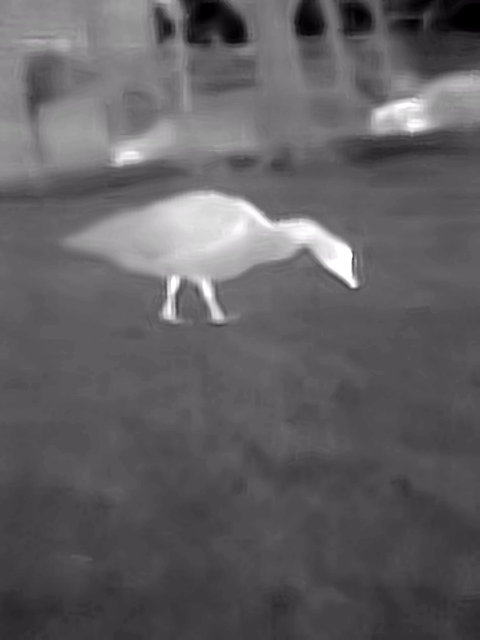
\includegraphics[width=\textwidth, trim={0cm 2.5cm 0cm 2.5cm}, clip]{images/dataset/goose/lwir.png}
    \caption{Goose}
  \end{subfigure}
  \caption{Example images for each class in the final dataset. Images have been cropped vertically.}
  \label{fig:dataset_classes}
\end{figure}

Figure \ref{fig:dataset_classes} shows example RGB and LWIR images from the training dataset. While these examples are sampeled from the "ideal" \textit{single} subsets, they highlight another important caveat. Not all images were captured at the same distance. Consequently, different animals fill different amounts of space within the images, possibly skewing classification results. An attempt was made to mitigate this issue through affine data agumentation.

\subsection{Data augmentation}

Due to the limited amount of time and resources available to the project, generating a dataset with sufficient scope and size is challenging. Since the performance of machine learning models is usually directly tied to the size and quality of the available dataset, an insufficient dataset might make it impossible to train an accurate and robust classifier \citep{fawzi_adaptive_2016}. Therefore, data augmentation will have to be employed to artificially increase the amount of usable training samples.

\citet{mikolajczyk_data_2018} make the distinction between white-box and black-box data augmentation methods. While the latter use a form of deep learning, namely Generative Adversarial Networks (GAN), to synthesise new training samples, white-box methods involve more traditional techniques, such as affine transformations. An affine transformation or affine map can accurately represent a composition of a translation and a linear map (e.g. scaling, rotation and shearing). A transformation $f(\vec{x})$ can be expressed as follows:

\begin{equation}
  f(\vec{x}) = A \vec{x} + \vec{b},
  \label{eqn:affine}
\end{equation}

where $\vec{x}$ represents the coordinates of a point to be translated, $A$ is a $2 \times 2$ linear map, and $\vec{b}$ is the translation vector. $f(\vec{x})$ can be applied to the coordinates $\vec{x}$ of every pixel, yielding a transformed image. If necessary, interpolation strategies are used to fill in gaps between the new pixels.

After evaluating various methods of data augmentation on a subset of the ImageNet dataset, \citet{perez_effectiveness_2017} conclude that traditional affine transformations alone can be very effective, although GAN-based methods are promising and might yield better results.

Due to the relatively easy implementation, this project therefore primarily uses white-box data augmentation. However, the design and implementation of a deep-learning model generating LWIR from visible light images is discussed in Section \ref{autoencoder_implementation}. This model could be used to generate new LWIR data samples from visible light images retrieved from other sources, such as existing computer vision datasets.

Figure \ref{fig:augmentation_affine} shows different affine transformations that were used to augment the captured dataset. The most natural transformation in this scenario is a horizontal flip, as we can assume that the objects to be classified are symmentric along the horizontal axis and the images have all been captured with similar camera orientations. Moreover, we employed randomized zooms to try to account for the varying distances that the animals were photographed from. We decided to limit the zoom factor to a small enough range to guarantee that the images still showed the whole object. Finally, we applied random rotations in the range from $-20^{\circ}$ to $20^{\circ}$ to account for slightly different camera orientations.

\begin{figure}[ht]
  \centering
  \begin{subfigure}[h!]{0.24\textwidth}
    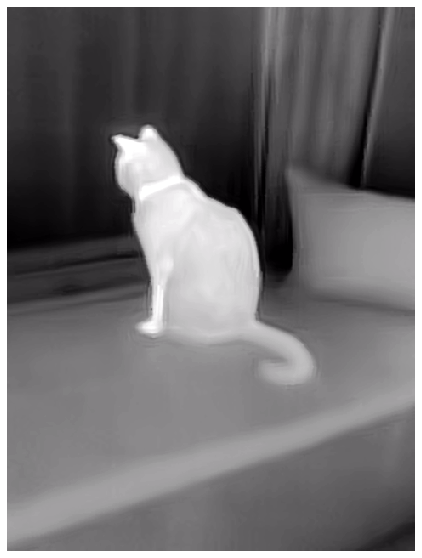
\includegraphics[width=\textwidth]{images/augmentation/original.png}
    \caption{Original image}
  \end{subfigure}
  \begin{subfigure}[h!]{0.24\textwidth}
    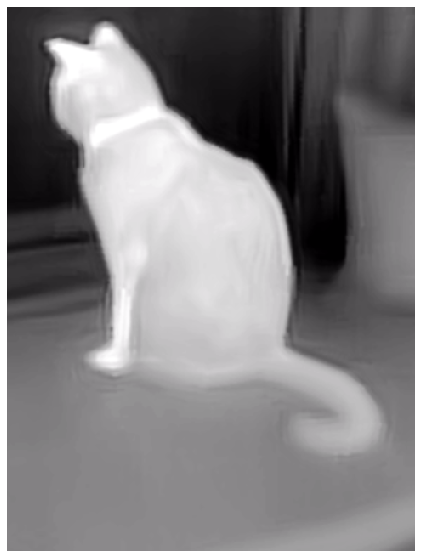
\includegraphics[width=\textwidth]{images/augmentation/zoomed.png}
    \caption{Zoomed in}
  \end{subfigure}
  \begin{subfigure}[h!]{0.24\textwidth}
    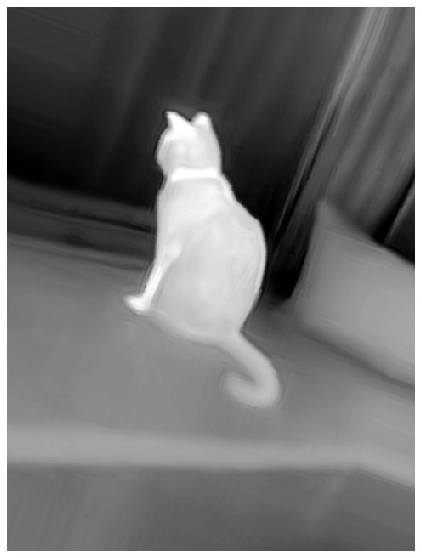
\includegraphics[width=\textwidth]{images/augmentation/rotated.png}
    \caption{Rotated $20^{\circ}$}
  \end{subfigure}
  \begin{subfigure}[h!]{0.24\textwidth}
    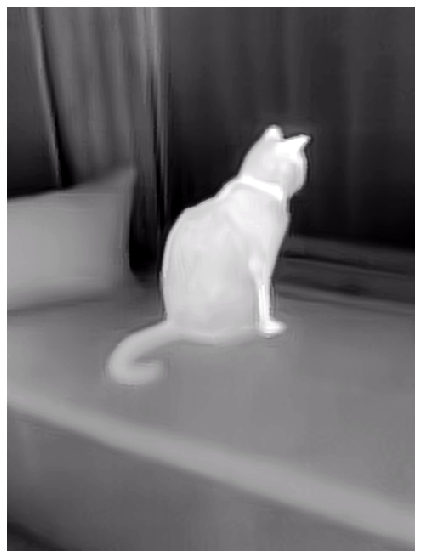
\includegraphics[width=\textwidth]{images/augmentation/flipped.png}
    \caption{Horizontally flipped}
  \end{subfigure}
  \caption{Affine data augmentation strategies applied to a sample LWIR image.}
  \label{fig:augmentation_affine}
\end{figure}

Another possible way of augmenting the data before classification is artificially drawing obstacles over the images. This approach could possibly help the model generalise better on the dataset, as a significant amount of samples from certain classes is obstructed by metal grids or foliage. However, this would require further investigation into the varying properties of visible light and LWIR images, and their interaction with different types of obstacles. Hence, this approach was not implemented in this project. Instead, we decided to remove a significant part of obstructed samples from the final dataset and focused on working with higher-quality data. 


%----------------------------------------------------------------------------------------------------------------------------------

\section{Image registration}
\label{image_registration}

The images captured by the visible light camera and thermal sensor of the FLIR One Pro are not properly aligned by default. This can have adverse consequences to the classification performance of a machine learning model (XXX citation needed). Thus, an algorithm for properly aligning the images captured by the conventional camera and LWIR camera had to be developed. The process of transforming data from different sensors into one coordinate system is commonly referred to as image registration.

On superficial inspection, it is apparent that the LWIR sensor appears to have a narrower field of view than the RGB camera. Hence, an attempt was made to manually align the LWIR and RGB images by cropping and rescaling the RGB image, effectively zooming in. This approach yielded moderate results, as can be seen in Figure \ref{fig:linear_trans_before_after}.

To obtain a more flexible and generalisable representation, we made use of affine transformations. As demonstrated in Equation \ref{eqn:affine}, an affine transformation can be expressed as a linear function with parameters $A$ and $\vec{b}$. These parameters can be easily trained using a linear regression model. Therefore, the coordinates of about a dozen reference points were manually determined on the RGB and LWIR versions of some test images. These coordinates were used as the inputs and outputs to train the aforementioned linear regression model. 

% The effect of applying the resulting transformation to a set of coordinates are shown in Figure \ref{fig:transformation_arrows}.

% \begin{figure}[ht]
%   \centering
%   \begin{subfigure}[h!]{0.45\textwidth}
%     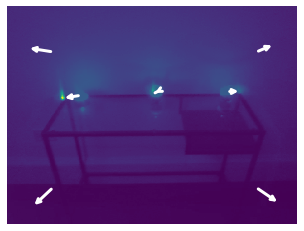
\includegraphics[width=\textwidth]{images/registration/transformation_arrows.png}
%     \caption{Synthetic image, black on white.}
%     \label{fig:transformation_arrows}
%   \end{subfigure}
%   \caption{}
% \end{figure}

\begin{figure}[ht]
  \centering
  \begin{subfigure}[h!]{0.3\textwidth}
    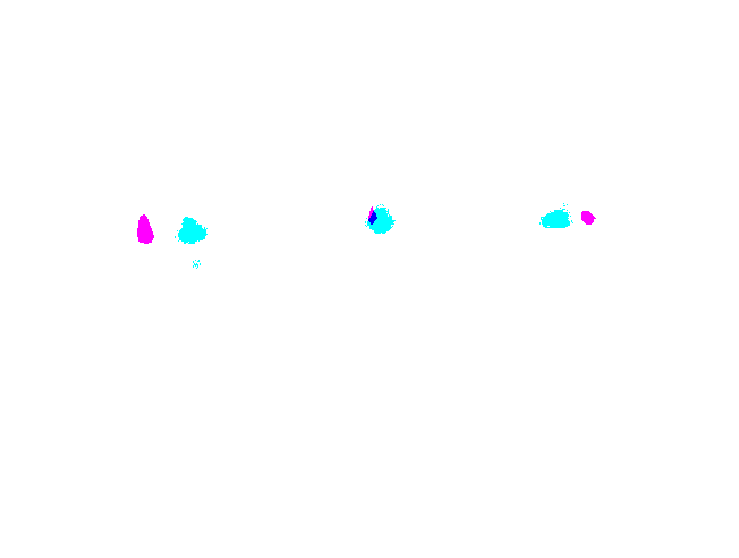
\includegraphics[width=\textwidth, trim={3.5cm 9cm 3.5cm 4.5cm}, clip, frame]{images/registration/unregistered.png}
    \caption{Before registration. The LWIR and VIS images are visibly misaligned.}
  \end{subfigure}
  \begin{subfigure}[h!]{0.3\textwidth}
    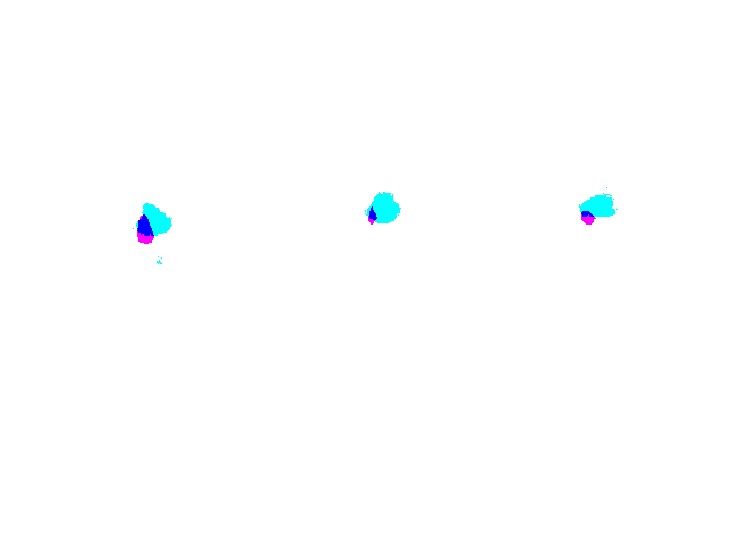
\includegraphics[width=\textwidth, trim={3.5cm 9cm 3.5cm 4.5cm}, clip, frame]{images/registration/registered_zoom.png}
    \caption{After zooming in. The images are almost aligned. A slight offset remains.}
  \end{subfigure}
  \begin{subfigure}[h!]{0.3\textwidth}
    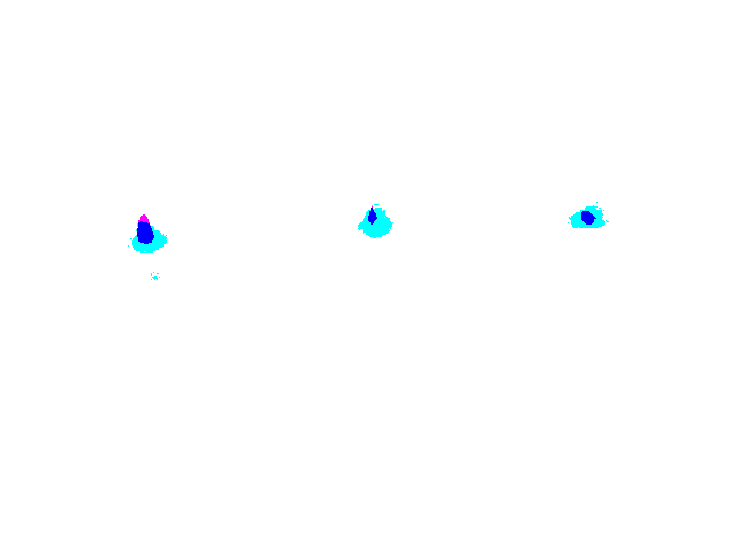
\includegraphics[width=\textwidth, trim={3.5cm 9cm 3.5cm 4.5cm}, clip, frame]{images/registration/registered_affine.png}
    \caption{After registration. The thermal signatures of the candles align with the VIS location.}
  \end{subfigure}
  \caption{Superimposed LWIR and VIS images before and after registration. All images have been thresholded.}
  \label{fig:linear_trans_before_after}
\end{figure}

This approach yielded acceptable results. As can be seen in Figure \ref{fig:linear_trans_before_after}, the candles in the images line up. Note that the images have been thresholded to better show the alignment of the reference points. The cyan channel represents the grayscale version of the visible light image and the magenta channel represents the LWIR image.

However, defining reference points manually is a time-consuming task and the quality of alignment is dependent on the precision of those points. To quantify the accuracy of the alignment, attempts were made to use various metrics for image similarity. Such metrics could be used as loss functions for a machine learning model to automatically align the channels.

This task is difficult, as the properties of objects are vastly different under visible light and far infrared. Therefore, a simple intensity-based metric is unlikely to be successful in this scenario, as local intensities will vary across different channels even if the registration is perfect \citep{myronenko_intensity-based_2010}.

\subsection{Intensity-based registration metrics}

To mitigate the problem of varying intensities across different channels, \citet{chen_normalized_2018} introduce the Normalized Total Gradient (NTG) metric for multispectral imaging systems, which is defined as follows:

\begin{equation}
  NTG(f, f_R) = \frac{\sum_l |\nabla_l \{f - f_R\}|}{\sum_l | \nabla_l f | + \sum_l | \nabla_l f_R|},
\end{equation}

where $f$ and $f_R$ are the channel images to be compared, $\nabla_l$ represents the gradient computation along the direction $l \in \{x, y\}$, and $| \cdot |$ denotes the L1-norm.

In other words, to obtain NTG one computes the sum of the $x$- and $y$-gradients of the difference of the two channels, and normalises the result by dividing over the sum of gradients of the individual channels.

The metric is based on the assumption that the gradient of the channel difference image becomes sparser as the alignment improves. Figure \ref{fig:gradient_distribution} shows that this is hardly the case for images captured by the LWIR camera, as opposed to the baseline of comparing the red and green channels from the RGB camera.

The resolution of the LWIR images, as output by the FLIR camera, is $640 \times 420$ px, although the actual resolution of the sensor is only $160 \times 120$. Thus, when downsampling the RGB image to $640 \times 420$ px, edges are still much sharper than for the corresponding LWIR image. Downsampling both images to the native resolution of the LWIR camera did not yield better results.

Moreover, an attempt at smoothing both images before calculating the NTG was made by applying the Laplacian of Gaussian (LoG) with $\sigma=2$ to both images. As can be seen in Table \ref{table:registration_ntg}, this approach was not successful either. To verify that our implementation of the metric was indeed working correctly, we computed the NTG between the red and green channel of the visible light image before and after applying a random affine transformation to the green channel. It can be seen that the metric is very effective for the red-green-channel baseline. 

Considering the results, it can be concluded that NTG is not a suitable metric for this particular problem. 
Since this is not the case for the baseline, it is possible that the properties of the LWIR and RGB channels are too different for an intensity-based approach.

\begin{figure}[ht]
  \centering
  \begin{subfigure}[h!]{0.45\textwidth}
    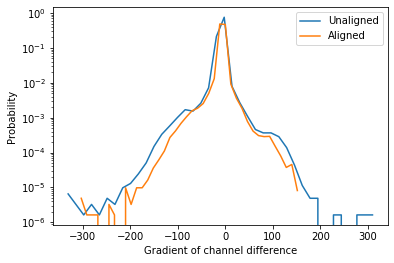
\includegraphics[width=\textwidth]{images/registration/gradient_distribution.png}
    \caption{LAB intensity of visible light image vs thermal intensity at $640 \times 420$ px}
    \label{fig:gradient_distribution}
  \end{subfigure}
  \begin{subfigure}[h!]{0.45\textwidth}
    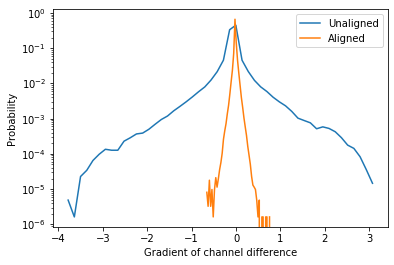
\includegraphics[width=\textwidth]{images/registration/gradient_distribution_red_green.png}
    \caption{Red channel intensity vs green channel intensity at $640 \times 420$ px}
    \label{fig:gradient_distribution_red_green}
  \end{subfigure}
  \caption{Distribution of gradients of the channel difference image before and after alignment using affine transformation.}
\end{figure}


\begin{table}[ht]
  \centering
  \begin{tabular}{@{}lll@{}}
  \toprule
  \textbf{Test configuration}                             & \textbf{Misaligned} & \textbf{Aligned} \\ \midrule
  LAB intensity of VIS vs LWIR (640x480)     & 0.9984              & 0.9987           \\
  LAB intensity of VIS vs LWIR (160x120)    & 0.9974              & 0.9986           \\
  LAB intensity of VIS vs LWIR (after LoG with $\sigma=2$) & 0.9970              & 0.9973           \\
  (Baseline) Red vs green channels of RGB (160x120)                  & 0.6245              & 0.0303           \\ \bottomrule
  \end{tabular}
  \caption{Normalized Total Gradient before and after channel alignment}
  \label{table:registration_ntg}
\end{table}


\subsection{Texture-based registration}

Having demonstrated that intensity-based metrics appear to be inadequate to quantify the registration of visible light and LWIR images, an approach based on image texture features, as proposed by \citet{jarc_graz_2007} was tested. 

The method uses pairs of 1-D filter masks as introduced by \citet{laws_rapid_1980} to detect level, edge, spot and ripple features. These filters can be applied horizontally and vertically. In our implementation, all possible filter pairs were evaluated.

After convoluting both the LWIR and RGB images with the filters, the results were turned into texture energy images by performing a convolutional sum-operation of absolute values using a $15 \times 15$ kernel and applying a threshold of $\pm 3 \sigma$. Figure \ref{fig:le_filter} shows corresponding VIS and LWIR images after applying the level kernel horizontally and the edge kernel vertically.

\begin{figure}[ht]
  \centering
  \begin{subfigure}[h!]{0.3\textwidth}
    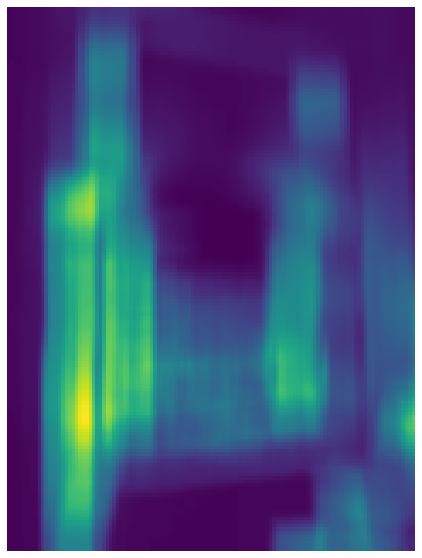
\includegraphics[width=\textwidth]{images/registration/filtered_le_rgb.png}
    \caption{VIS}
  \end{subfigure}
  \begin{subfigure}[h!]{0.3\textwidth}
    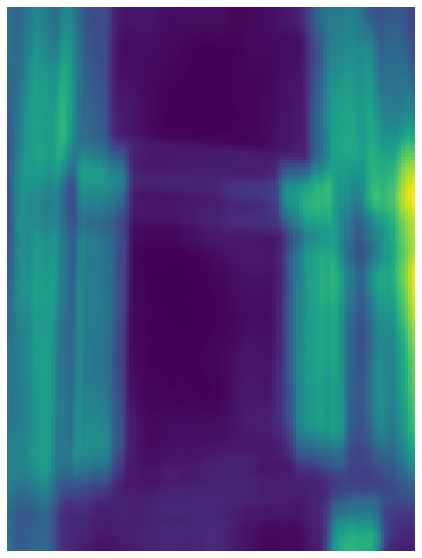
\includegraphics[width=\textwidth]{images/registration/filtered_le_lwir.png}
    \caption{LWIR}
  \end{subfigure}
  \caption{Effect of LE-Kernel \citep{laws_rapid_1980} on visible light and LWIR images.}
  \label{fig:le_filter}
\end{figure}

Finally, the mutual information (MI) of the resulting LWIR and RGB images was calculated as follows:

\begin{equation}
  MI(A,B) = H(A) + H(B) - H(A,B),
\end{equation}

where $H(X) = - \sum_{x \in X} p(x) \cdot \log_2 p(x)$ is the entropy of $X$ and $H(X,Y)$ represents the joint entropy of $X$ and $Y$.

We then averaged the MI scores obtained by all 1-D filter pairs to obtain a single metric. For the test images, the MI score did not appear to change consistently when aligning the images. Furthermore, none of the MI values for the different filter combinations behaved reliably across all images. 


\subsection{Mean squared distance}

Since neither intensity-based, nor texture-based approaches produced satisfactory results, we concluded that automatic alignment of the visible light and LWIR images is unfeasible without extensive further research. Therefore, to be able to guarantee an acceptable alignment quality, we resorted to the aforementioned manual approach.

XXX reference points in XXX images were recorded and the corresponding transformation matrix was determined. Prior experiments showed that the required transformation matrix seems to be mostly constant across different images. Device orientation seemed to be the only factor with a large impact on the required transformation. To avoid this problem, all images were captured in portrait mode.

The mean squared distance (MSE) across all reference points in the dataset was determined to be XXX.

%----------------------------------------------------------------------------------------------------------------------------------

\section{Classifiers}

As concluded in \ref{fig:augmentation_affine}, the spatial and intensity properties of RGB and LWIR images are significantly different. Consequently, we decided to implement five versions of every CNN and evaluate the results separately.

\begin{enumerate}
  \item An RGB-only implementation similar to the default implementation of most networks. This will be used as a baseline.
  \item An LWIR-only implementation.
  \item A greyscale implementation. This will calculate the mean across the three colour channels of the RGB image, yielding a single-channel greyscale image. The purpose of this model will be to evaluate the benefits and drawbacks of using all three colour channels.
  \item A single-branch, stacked-layer implementation. The RGB and LWIR channels are stacked into a tensor of shape $({batch_size} \times width \times height \times 4)$. This tensor is then fed into the network, yielding a prediction.
  \item A multi-branch implementation with late feature fusion. Here, the RGB and LWIR images are fed into separate branches of hidden layers. Finally, the respective outputs are being flattened, concatenated and fed into the fully-connected layers at the end of the network.
  \item A multi-branch implementation with voting classifiers. Similarly to the late feature-fusion implementation, the images are run through seperate branches. However, the branches have their own individual fully-connected layers, which produce separate predictions. The final output is the weighted mean of these two predictions. 
\end{enumerate}

This project will therefore attempt to evaluate the performance of early feature-fusion, late feature-fusion and voting classifiers. We chose the RGB-only networks as a baseline, as most image classification models rely solely on visible light.

\subsection{AlexNet}

AlexNet was first introduced by \citet{krizhevsky_imagenet_2012}.

Our implementation of AlexNet diverges slightly from the original in several points.

\begin{figure}[ht]
  \centering
  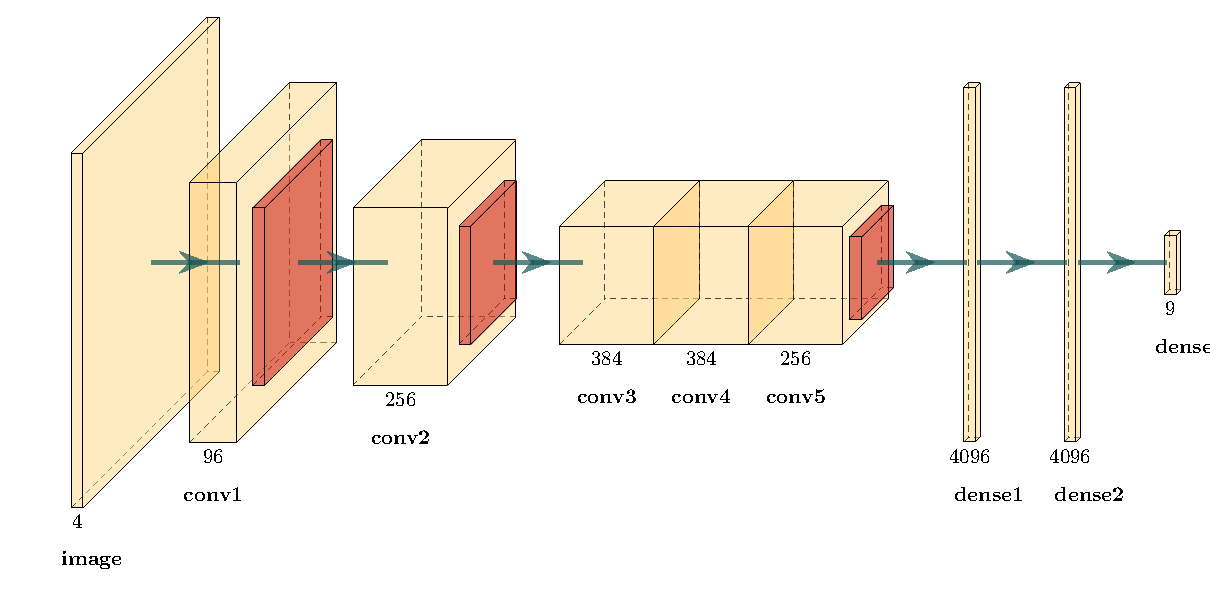
\includegraphics[width=0.9\textwidth]{images/models/alexnet}
  \caption{Neural network architecture of AlexNet.}
  \label{fig:alexnet}
\end{figure}

%----------------------------------------------------------------------------------------------------------------------------------


\section{Mobile application}

The mobile application was designed with two primary requirements in mind:

\begin{itemize}
  \item Enabling the easy capture of combined visible-light and thermal datasets.
  \item Being able to perform live multi-class classification on multiple species of animals.
\end{itemize}



%==================================================================================================================================
\chapter{Implementation}
What did you do to implement this idea, and what technical achievements did you make?

\section{Data augmentation}

\subsection{Affine data augmentation}

Various libraries and tools are available to perform real-time data augmentation as part of the training pipeline. However, to achieve the highest possible level of control, a custom data augmentation function was designed. It leverages Tensorflow's ImageDataGenerator to apply random affine transformations to images in the dataset.

The script works by counting the number of samples per class and determining the class with the highest support. Each sample in that class is then augmented $n$ times. Finally, all remaining classes are being augmented until their sample size reaches that of the max class. The aim of this algorithm is to provide an even dataset without class imbalances.


\subsection{Predicting LWIR images using an autoencoder}
\label{autoencoder_implementation}

\subsubsection{Traditional autoencoder}

A deep convolutional autoencoder was created to predict the LWIR signature of objects from the corresponding visible light image. The architecture of the network is shown in Figure \ref{fig:autoencoder_architecture}. The network consists of an encoder and a decoder that each contain four blocks of layers.

Each encoder block has a convolutional layer, followed by a leaky ReLU activation function and a subsequent max pooling layer for downsampling. The $320 \times 240 \times 1$ input images are thus processed and downsampled to a $20 \times 15 \times 32$ tensor containing a compact, latent representation of the features in the original image.

The output of the decoder is then fed forward into four blocks of deconvolutional layers followed by leaky ReLU activation to attempt a reconstruction the LWIR image. Each deconvolutional layer tries to upsample the input by predicting appropriate pixel values.

For this task, a subset of the animals dataset with 336 images of Shetland ponies was chosen. Mean squared error was selected as the loss function. The network was trained for 100 epochs with a batch size of 16. Training time averaged around 18 minutes on an NVIDIA Tesla P-100 GPU.

After successful training of the network, two images of ponies were retrieved from Wikimedia Commons. They were then fed into the network in an attempt to generate the corresponding LWIR images. The output of the autoencoder can be seen in Figure \ref{fig:autoencoder_pony}.

\begin{figure}[ht]
  \centering
  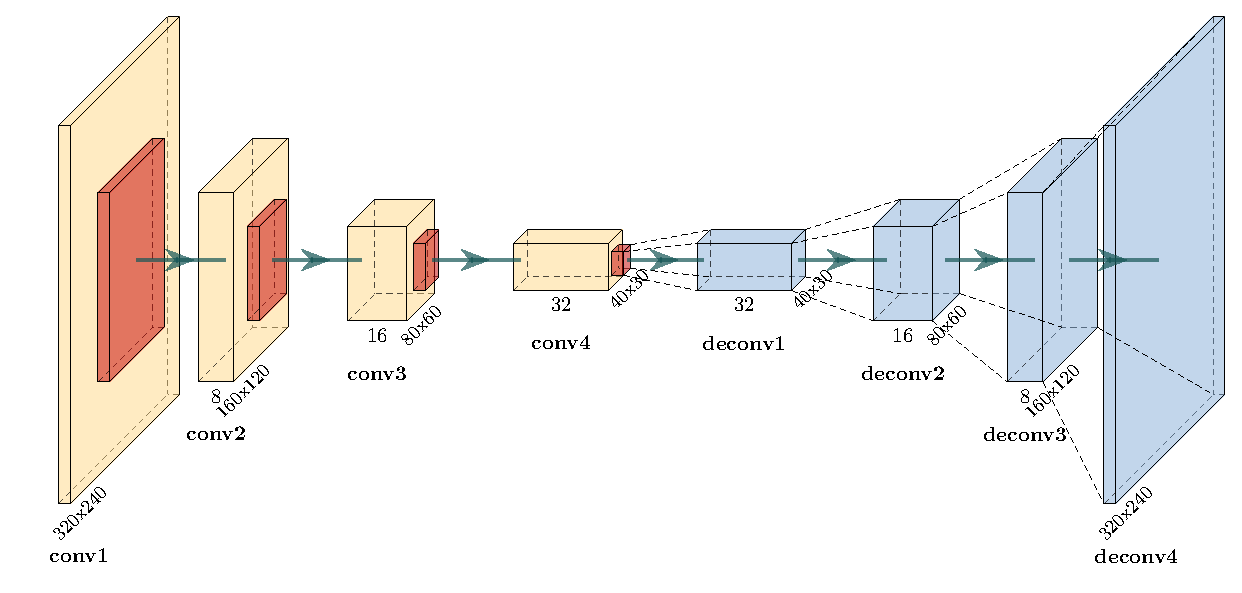
\includegraphics[width=0.9\textwidth]{images/autoencoder/autoencoder}
  \caption{Neural network architecture of the autoencoder.}
  \label{fig:autoencoder_architecture}
\end{figure}

\subsubsection{U-Net}

U-Net was first introduced by \citet{ronneberger_u-net_2015} to improve performance of biomedical image segmentation systems. Similarly to a conventional autoencoder, it features a contracting path that downsamples or encodes the input, and a symmetric expanding path that upsamples or decodes the input. Additionally, for each deconvolutional layer, the output of the corresponding opposite convolutional layer is concatenated to the layer's input map. These connections can be seen in Figure \ref{fig:unet_architecture}. 

Similar to the traditional autoencoder, the U-Net was trained for 100 epochs on the the same dataset. Figure \ref{fig:autoencoder_pony} shows the output of the U-Net and compares it to the autoencoder output.



\begin{figure}[ht]
  \centering
  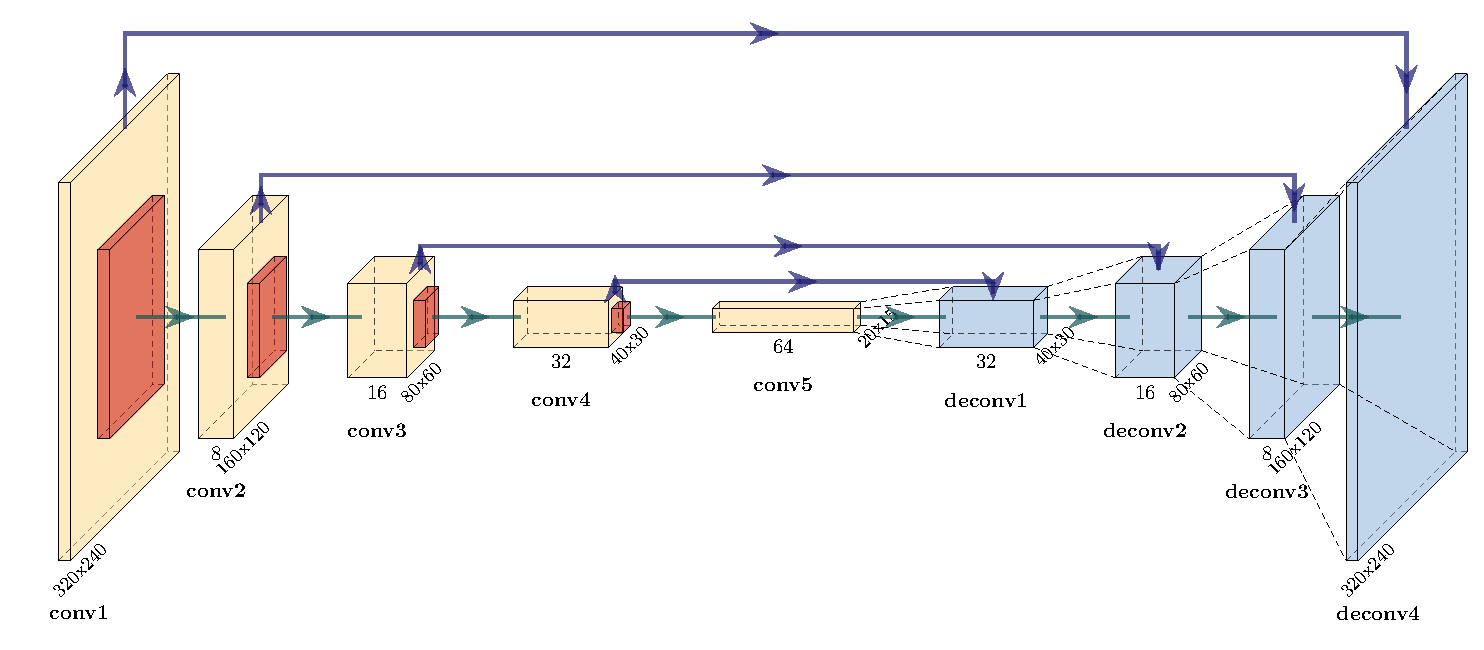
\includegraphics[width=0.9\textwidth]{images/unet/unet}
  \caption{Neural network architecture of the U-Net.}
  \label{fig:unet_architecture}
\end{figure}

\begin{figure}[ht]
  \centering
  \begin{subfigure}[h!]{0.25\textwidth}
    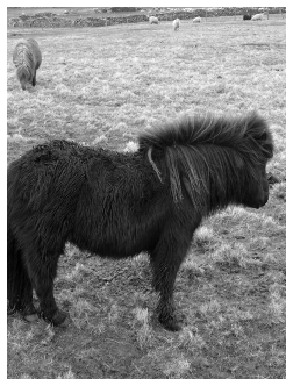
\includegraphics[width=\textwidth]{images/unet/pony_grayscale.png}
    % 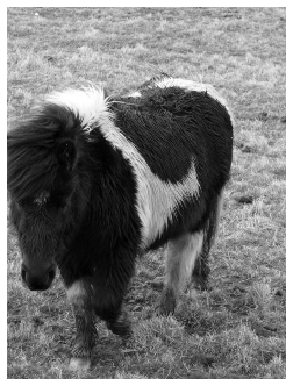
\includegraphics[width=\textwidth]{images/unet/pony_2_grayscale.png}
    \caption{Original images (cropped)}
  \end{subfigure}
  \begin{subfigure}[h!]{0.25\textwidth}
    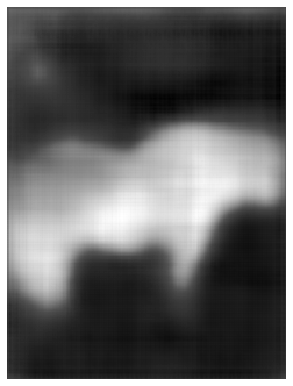
\includegraphics[width=\textwidth]{images/autoencoder/pony_predicted.png}
    % 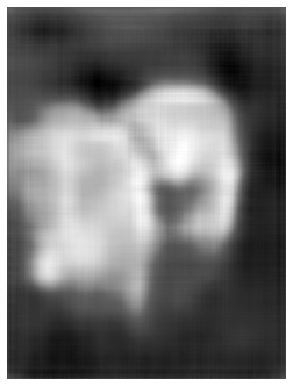
\includegraphics[width=\textwidth]{images/autoencoder/pony_2_predicted.png}
    \caption{Autoencoder prediction}
  \end{subfigure}
  \begin{subfigure}[h!]{0.25\textwidth}
    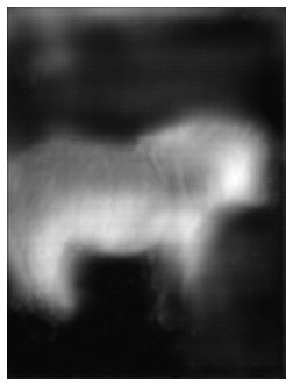
\includegraphics[width=\textwidth]{images/unet/pony_predicted.png}
    % 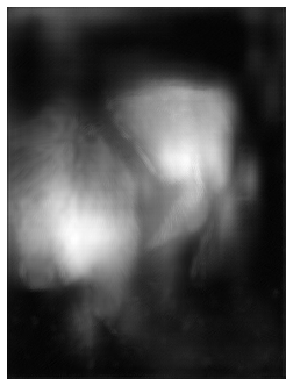
\includegraphics[width=\textwidth]{images/unet/pony_2_predicted.png}
    \caption{U-Net prediction}
  \end{subfigure}
  \caption{Predicted LWIR signature of images of shetland ponys. Retrieved from \url{https://commons.wikimedia.org/wiki/File:Sandwick_Shetland_Pony.jpg} and \url{https://commons.wikimedia.org/wiki/File:Shetland_ponies_at_Sandwick.jpg}}
  \label{fig:autoencoder_pony}
\end{figure}




% \begin{figure}[ht]
  %   \centering
  %   \begin{subfigure}[h!]{0.3\textwidth}
    %     \includegraphics[width=\textwidth]{images/autoencoder/mirror/grayscale.png}
    %     \caption{Grayscale of visible light}
    %     \label{fig:gradient_distribution}
  %   \end{subfigure}
  %   \begin{subfigure}[h!]{0.3\textwidth}
    %     \includegraphics[width=\textwidth]{images/autoencoder/mirror/pred_fir.png}
    %     \caption{Predicted LWIR}
    %     \label{fig:gradient_distribution_red_green}
  %   \end{subfigure}
  %   \begin{subfigure}[h!]{0.3\textwidth}
    %     \includegraphics[width=\textwidth]{images/autoencoder/mirror/actual_fir.png}
    %     \caption{Actual LWIR}
    %     \label{fig:gradient_distribution_red_green}
  %   \end{subfigure}
  %   \caption{Autoencoder prediction of LWIR image from grayscale.}
% \end{figure}

\section{Classification}

\subsection{Data loading}

Google Colaboratory was used throughout the majority of the project. Due to the limited amount of memory Colab provides, it was impossible to pre-load the entire training dataset into memory for training. For this reason, a data loader class was implemented that supported lazy loading of data batches. When constructing the loader, a batch size can be specified, in addition to whether image samples shall be registered, and the target image resolution. 

Since the data loader extends Keras' Sequence class, it fully integrates with the Model training API. When constructed, it loads a list of all samples, containing image paths and class labels. It then enumerates the classes.

When \lstinline{model.fit()} is called with the data loader as data source, Keras will call the \lstinline{__getitem__()} function repeatedly to lazily load batches of data into memory. The data loader will load the images in a batch, register them if demanded, and convert them into a tensor of shape $(batch size \times height \times width \times channels)$. Finally, it will return a tuple containing the image tensor and the one-hot representation of the numeric class labels.

While this approach was necessary to fit the model on the whole training dataset, we found that it noticably slowed down training speeds. This is most likely due to slow I/O bottlenecking the loading speed. An attempt was made to use Tensorflow's data API instead of OpenCV for loading and pre-processing to load the data directly into VRAM. However, the performance improvement was negligible.

\subsection{Models}



\section{Mobile application}

The mobile application was implemented using Java and Android Studio. 



%==================================================================================================================================

\chapter{Evaluation} 
How good is your solution? How well did you solve the general problem, and what evidence do you have to support that?

\section{Methods and hyperparameters}

\subsection{Data augmentation}

\subsection{Training-validation split}
\label{eval_train_val_split}

Multiple configurations of train/test split were attempted. Splitting the data with stratified sampling and train-test-split of 80-20, all models nearly achieved perfect classification accuracy. Figure \ref{fig:conf_stratified} shows the confusion matrix of the XXX classifier.  

\begin{figure}[ht]
  \centering
  \begin{subfigure}[h!]{0.4\textwidth}
    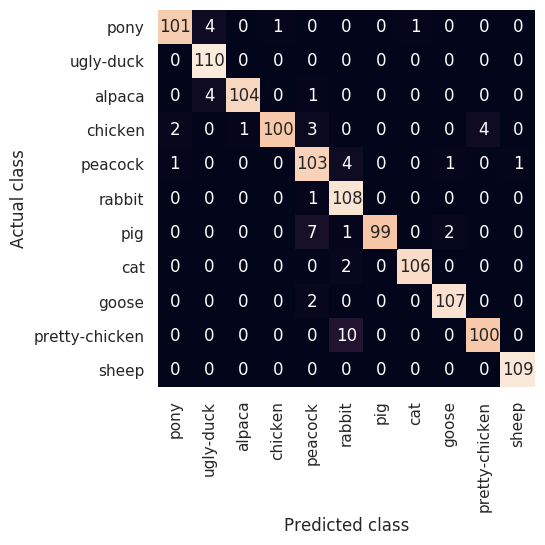
\includegraphics[width=\textwidth]{images/evaluation/confusion/vis_fir_confusion.png}
    \caption{Stratified sampling}
    \label{fig:conf_stratified}
  \end{subfigure}
  \begin{subfigure}[h!]{0.4\textwidth}
    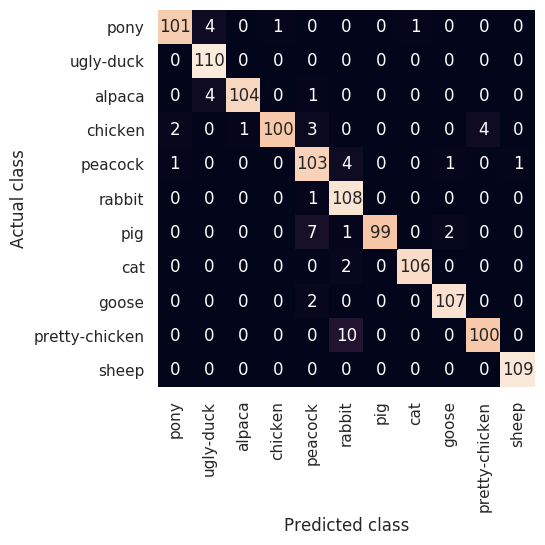
\includegraphics[width=\textwidth]{images/evaluation/confusion/vis_fir_confusion.png}
    \caption{Manual split (Section \ref{classes_samples})}
    \label{fig:conf_stratified}
  \end{subfigure}
  \caption{Confusion matrices for differnt train-validation splits.}
\end{figure}

This result is most likely due to the similarity of many images as mentioned in Section XXX. Since train and test samples are drawn from the same raw dataset, we conclude that it is very likely that the models are significantly overfitted on the captured data. It is unlikely that they would perform as well on chaotic new data as indicated by the validation accuracy.

Fitting the models on the training dataset as defined in Section \ref{classes_samples}, validation scores dropped significantly. This was in accordance with our expectations, as the samples from the training and validation datasets should now be independent. Therefore, the models are not able to overfit on the whole dataset anymore and the validation score is more representative of potential performance on new data.

\subsection{Generation of artificial data}

\subsection{VIS only compared to VIS+LWIR}

%----------------------------------------------------------------------------------------------------------------------------------

\section{Different network designs}

\subsection{Custom CNN}

\subsection{AlexNet}

\subsection{ResNet}

%----------------------------------------------------------------------------------------------------------------------------------

\section{Computational performance on mobile device}


%==================================================================================================================================
\chapter{Conclusion}    
Summarise the whole project for a lazy reader who didn't read the rest (e.g. a prize-awarding committee).

%==================================================================================================================================
%
% 
%==================================================================================================================================
%  APPENDICES  

\begin{appendices}

\chapter{Appendices}

Typical inclusions in the appendices are:

\begin{itemize}
\item
  Copies of ethics approvals (required if obtained)
\item
  Copies of questionnaires etc. used to gather data from subjects.
\item
  Extensive tables or figures that are too bulky to fit in the main body of
  the report, particularly ones that are repetitive and summarised in the body.

\item Outline of the source code (e.g. directory structure), or other architecture documentation like class diagrams.

\item User manuals, and any guides to starting/running the software.

\end{itemize}

\textbf{Don't include your source code in the appendices}. It will be
submitted separately.

\end{appendices}

%==================================================================================================================================
%   BIBLIOGRAPHY   

% The bibliography style is abbrvnat
% The bibliography always appears last, after the appendices.

\bibliographystyle{abbrvnat}

\bibliography{l4proj}

\end{document}
